%% Copyright (C) 2009 by Tobias Elze
%% Journal of Vision LaTeX template version 1.0
%% This document may be used freely for your own submissions.

\documentclass{jov}
\usepackage{graphicx} % needed for figures
\usepackage{subcaption}
\usepackage{hyperref}
\usepackage{amsmath}
\usepackage{bbm}
\usepackage{amssymb}
\usepackage{comment}

\DeclareMathOperator*{\argmin}{arg\,min}

\begin{document}

\title{Luminance constancy under fixed geometry}
\abstract{The light that reflects off an object surface and is captured by our eyes varies significantly with its context. 
But, the human visual system has the ability to stably perceive the object's color invariant of the context variations. 
While this invariance detection ability is behaviorally very significant, its mechanism remains largely unknown. 
To understand the computational principles that lead to invariant color perception, 
here we study the perception of object light reflectance value (LRV) under variations in naturalistic scenes. 
Specifically, we study the effects of variations in reflectance and illumination spectra in a scene on the 
perceived LRV of a target object. 
We have developed a software that renders naturalistic multispectral images of 3D scenes.
The software provides precise control over the geometrical and spectral factors that make a scene. 
We label the rendered images with the luminance of a specific object in the scene. 
Next, we simulate the response of the retinal cones to these multispectral images using 
an accurate model of the early visual system. 
We then use supervised learning methods on these labeled cone responses to 
identify the computations that lead to accurate LRV estimation under changes in spectral condition. 
We show that if only either target or target and illumination spectra are allowed to vary, the standard luminance can be estimated through simple transformations of the cone responses. 
When all the spectra vary simultaneously, while it is not easy to recover the luminance through simple transformations, 
a decoding scheme that compares the light from the target and the surround, and properly adds the response of the L,M and  
S cones can recover the luminance within about 13\% RMSE.}

\author{Singh}{Vijay}
 {Computational Neuroscience Initiative}
 {and Department of Physics, University of Pennsylvania, PA, USA}
 {}{vsin@sas.upenn.edu}

\keywords{color constancy, luminance constancy, supervised learning}

\maketitle

\section{Introduction}
The perceived color of an object has important behavioral implications, since color helps to identify objects and their properties \cite{Mollon89, Jacobs81}.
[THIS PERCEIVED COLOR DEPENDS ON THE SURFACE REFLECTANCE OF THE OBJECT.]
Perceived object color is not sensed directly. Rather, it is computed by the brain starting with the retinal image of the light reflected from an object to the eye.
The computational challenge underlying object color perception is that this reflected light depends not just on the object's surface reflectance, but also on extrinsic factors such as the illumination, the object's pose, and the position of the observer (Fig.~\ref{fig:introSchematic}).
To produce a stable perceptual representation correlated with an object's surface reflectance the brain must account for these intrinsic factors on the reflected light.
The ability of a visual system to extract such a stable representation is called color constancy. 
[DO WE NEED THIS LINE -] Although human color constancy is by no means perfect, it is often very good \cite{FosterColorConstancy, BrainardColorConstancy}. 
In this paper, we consider the computational problem of color constancy, that is, how in principle could a visual system process the light reflected to the eye to produce percepts well-correlated with object surface reflectance.

Early work on computational color constancy considered a simplified case with multiple flat matte objects and a single spatially diffuse illuminant \cite{LandRetinex,Buchsbaum80,MaloneyWandell86}. Subsequent computational work considered more complex geometries and incorporated probabilistic descriptions of the statistics of naturally occurring scenes \cite{funt1988color, D'ZmuraConstancy3, barron2012color, D'ZmuraIversonSinger,BrainardFreeman}; LET'S SEE IF WE CAN FIND SOME RECENT REVIEWS).
A key insight from this computational work is that stable color descriptors of a target object cannot be obtained from the light reflected from the target object alone.  But, it is possible to obtain such descriptors by analyzing jointly the light reflected from all of the objects in the scene.
As a consequence, the performance of color constancy algorithms will be affected by variation in the surface reflectance of all of the objects in the scene \cite{BrainardWandellRetinex}, not just by variation in the illuminant. Thus evaluation of constancy algorithms must include assessment of their performance with respect to both variation in the illumination and the surface reflectance of all of the scene objects \cite{BrainardWandellRetinex,BrainardFreeman}. 

% Figure 1: Introduction
\begin{figure}
\centering
\begin{subfigure}{0.4 \textwidth}
	\centering
	\caption{}
        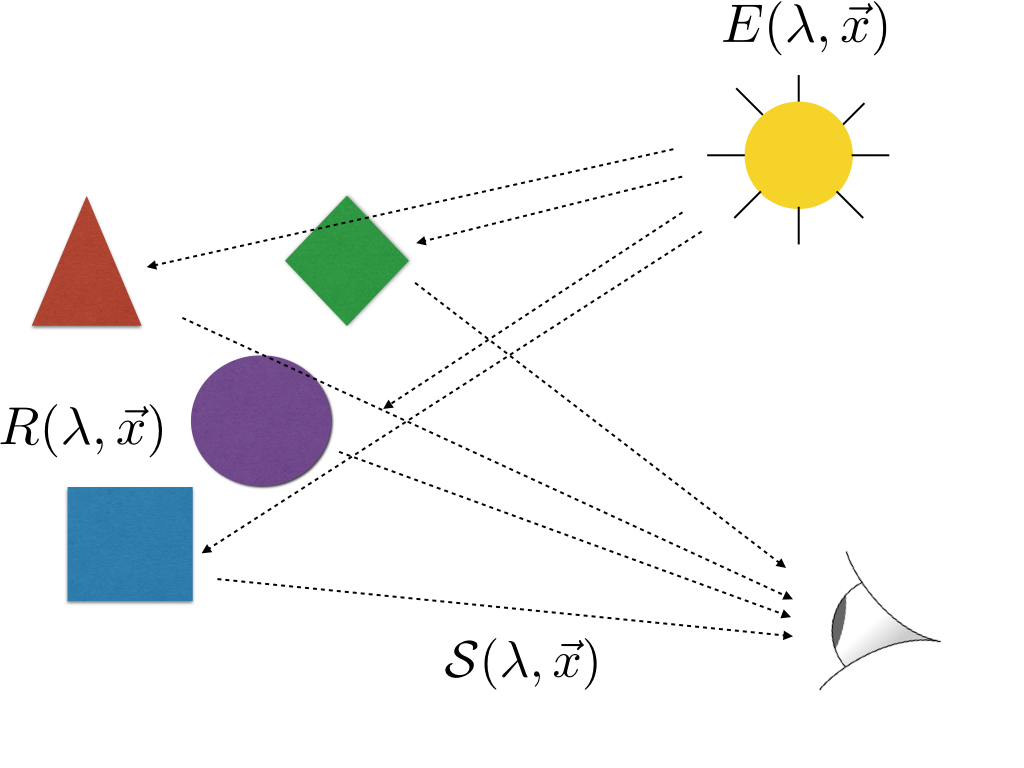
\includegraphics[width=\textwidth]{../FiguresDraft4/Figure1/Figure1_a.png}
        \label{fig:introSchematic}
    \end{subfigure}
    \begin{subfigure}{0.55 \textwidth}   
        \caption{}    
        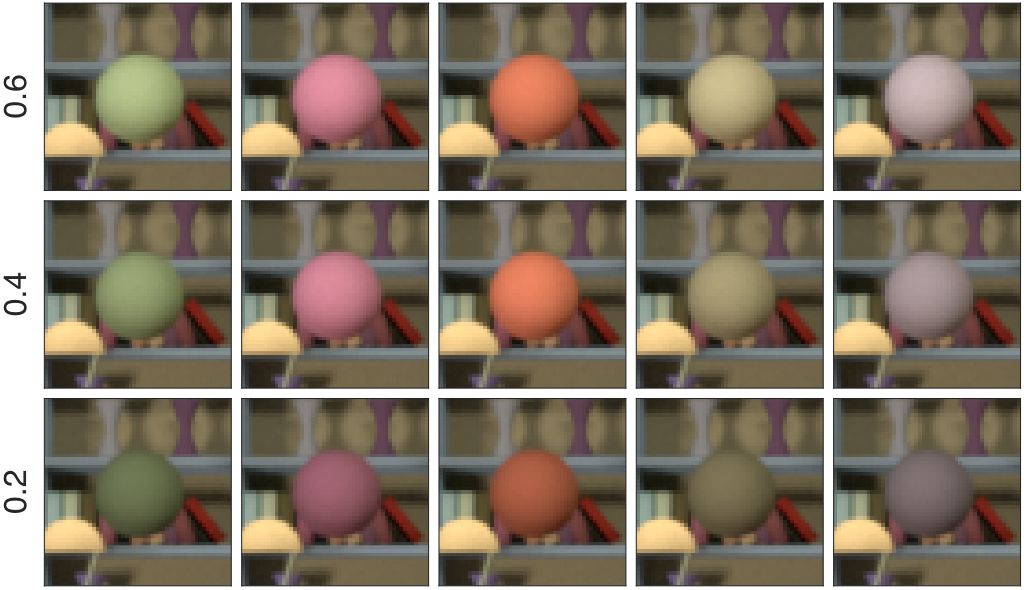
\includegraphics[width=\textwidth]{../FiguresDraft4/Figure1/Figure1_b.png}
        \label{fig:introExampleFigure}
    \end{subfigure}
    \label{introFigure}
    \caption{(a) {\bf Color Constancy:} The light reflected from an object to the eye depends both on the object's surface reflectance of the object and the illumination. It also depends on geometric factors, such as the object's shape, pose, and position relative to the observer. The human visual system is able to account for variations in the reflected light due to object-extrinsic factors and produce a percept of object color that is relatively stable, an ability called color constancy. (b) {\bf Luminance Constancy:} Images of a sphere under a fixed illuminant.  Down each column, the reflectance function of the sphere varies only by a scale factor; the relative reflectance spectrum held fixed.  The relative spectrum (shape of reflectance spectrum) varies across each row.
Within each row, the light reflectance value (LRV) of the spheres is constant. The values on the left of each row provide the corresponding LRV. We cast the problem of computational luminance constancy to be that of estimating LRV from the image, across variation in other scene factors: variation in relative surface reflectance, variation in illumination, and variation in the reflectance of the other objects in the scene.}
 \end{figure}

An alternative approach to computational color constancy, which has been less-well explored, is to use supervised machine learning techniques to develop mappings between input images and stable color descriptors \cite{barron2015convolutional}. The use of supervised learning to understand perceptual capabilities for natural stimuli has enjoyed success in domains outside of color vision. For example, a recently developed technique called accuracy maximization analysis (AMA) learns linear filters optimized for particular perceptual tasks \cite{geisler2009optimal}. It has been used to develop ideal observers for speed, focus error, and disparity estimation that provide excellent models of human performance \cite{burge2011optimal, burge2014optimal, burge2015optimal}. In this paper, we apply AMA to a special case of computational color constancy. 

Supervised learning requires large labeled data sets.  Such data sets are not readily available for the study of color constancy. Although there are databases of calibrated color images, these do not provide ground truth information about surface reflectance and illuminantion at each image location \cite{ChakrabartiHyperspectral,NascimentoFoster2016,ParragaHyperspectralData,TkacikUpennHypersepctralData,skauli2013collection,olmos2004biologically}. There are some smaller databases consisting of images of posed scenes where object surface reflectances are measured individually (\citeNP{funt1988color,ciurea2003large}; \citeauthor{davidPennHyperspectral}), but these are not large enough to drive supervised learning.
 
% Figure 2: Conditions Studied
\begin{figure}
\centering
	\begin{subfigure}[b]{0.33 \textwidth}
		\caption{Condition 2}
		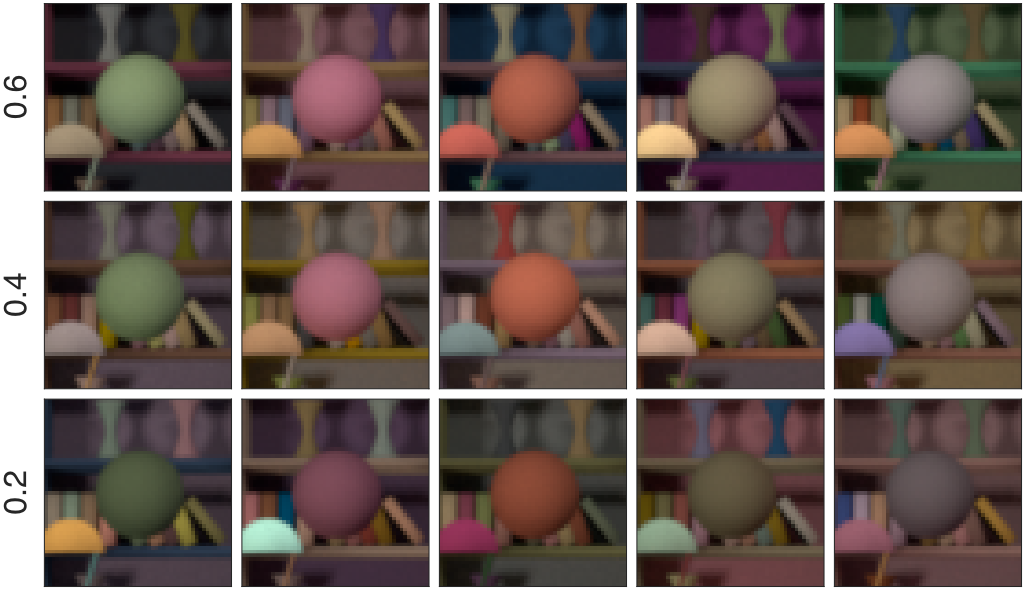
\includegraphics[width=\textwidth]{../FiguresDraft4/Figure2/Figure2_a.png}
 		\label{fig:backgroundVarying}
	\end{subfigure}
	\begin{subfigure}[b]{0.33 \textwidth}
        \caption{Condition 3}	
        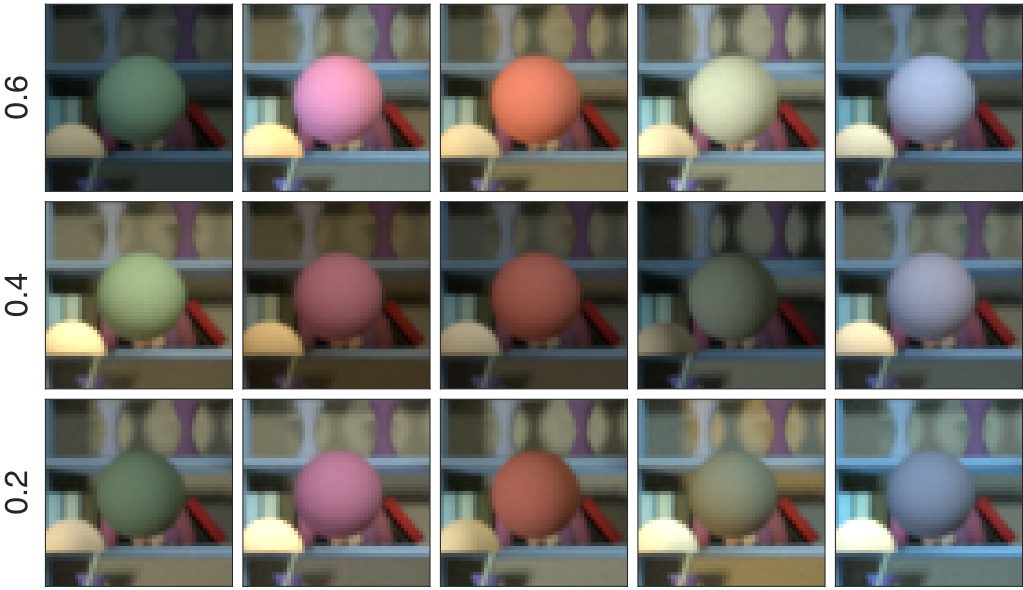
\includegraphics[width=\textwidth]{../FiguresDraft4/Figure2/Figure2_b.png}
        \label{fig:targetIlluminantVarying}
    \end{subfigure}
	\begin{subfigure}[b]{0.33 \textwidth}
	\caption{Condition 4}	
        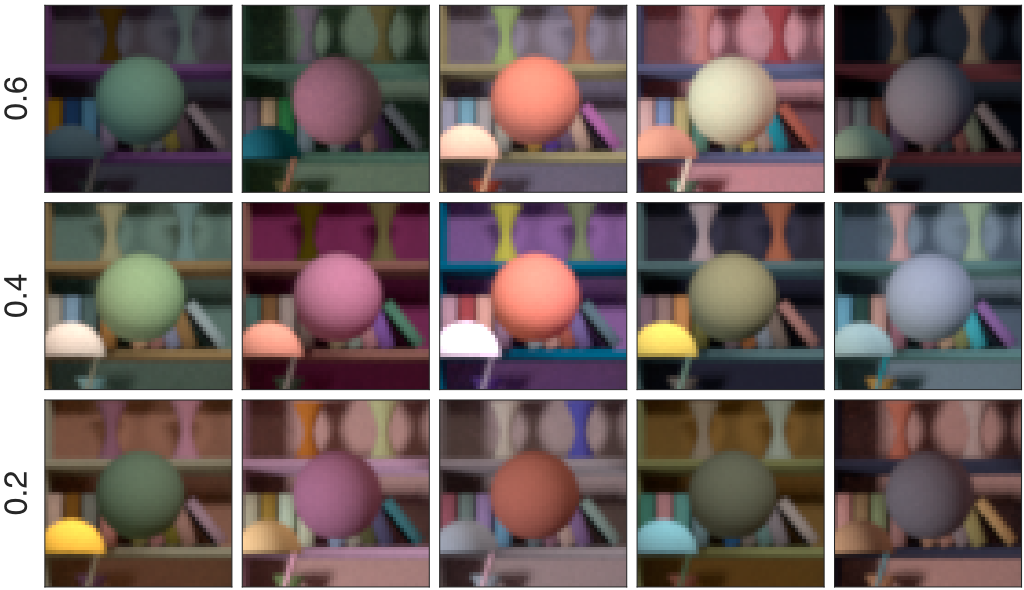
\includegraphics[width=\textwidth]{../FiguresDraft4/Figure2/Figure2_c.png}        
        \label{fig:allSpectraVarying}
    \end{subfigure}    
    \caption{{\bf Types of spectral variations studied in this work:} sRGB rendition of multispectral images similar to ones studied in our work. The numbers on the left indicate the standard luminance level of the target object. 5 images are shown at each luminance level. We studied four types of spectral variations. Condition 1: target object relative surface reflectance spectrum variable, light source spectra fixed, background object spectra fixed, (Fig.~\ref{fig:introExampleFigure}). (a) Condition 2: target object relative surface reflectance spectrum variable, light source spectra fixed, background object spectra variable, (b) Condition 3: target object relative surface reflectance spectrum variable, light source spectra variable, background object spectra fixed, (c) Condition 4: target object relative surface reflectance spectrum variable, light source spectra variable, background object spectra variable. As in Fig.~\ref{fig:introExampleFigure}, the spheres in each row of each panel have the same surface luminance, while the spheres in each column of each panel have the same relative surface reflectance.  Moreover, across the four panels (Fig.~\ref{fig:introExampleFigure} \& Fig.~\ref{fig:studiedCases}), spheres in corresponding locations have the same surface reflectance. In all four panels, the overall lights source spectra scale factors (see \nameref{Methods}) were drawn from a uniform distribution on the range [0.5, 1.5]. The sRGB values for all three panels were normalized using a common scale factor prior to gamma correction.} 
\label{fig:studiedCases}
\end{figure}

In this paper, we use high-quality computer graphics to generate large data sets of naturalistic images where the surface reflectance and illumination corresponding to each image pixel are known. 
This approach allows us to investigate computational color constancy with naturalistic stimuli, while retaining the ability to control the properties of objects and illuminants. Here, we use this approach to tackle luminance constancy, a constitutive component of the more general color constancy problem (Fig.~\ref{fig:introExampleFigure}). 

We define the computational problem of luminance constancy as that of estimating the light reflectance value (LRV) of an object's surface reflectance function.
The LRV is a measure of the overall amount of light reflected by a surface (\citeauthor{astm1121477}).
More precisely, the LRV is the luminance of the light that would
be reflected to the eye from an object with the specified surface reflectance function when the object is illuminated by a reference illuminant,
normalized by the luminance of the reference illuminant itself.
Here we use CIE daylight D65 as the reference illuminant and the CIE 1931 photopic luminosity function \cite{CIE86}.
LRVs are typically expressed in percent, so that they range from 0 to 100.

\section*{Methods} \label{Methods}
\subsection{Overview}
There are four key parts to our methods.  First we generate a labeled set of training images.  Second we use a model of the early visual system the compute the responses of the cone photoreceptor mosaic to the labeled images. Third we apply AMA to the cone responses to learn task-optimal receptive fields (RFs). Fourth we evaluate how well the responses of the RFs may be decoded to achieve luminance constancy.

\subsection{Labeled training data} \label{method:VirtualWorld}
% Figure 3
\begin{figure}[t]
\centering
\begin{subfigure}[b]{0.22 \textwidth}
        \caption{Library }
        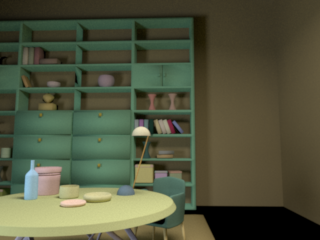
\includegraphics[width=\textwidth]{../FiguresDraft4/Figure3/Figure3_a.png}
        \label{fig:baseSceneLibrary}
    \end{subfigure}
    ~
    \begin{subfigure}[b]{0.22 \textwidth}
        \caption{Mill}    
        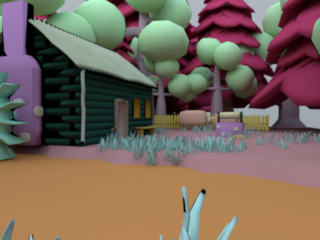
\includegraphics[width=\textwidth]{../FiguresDraft4/Figure3/Figure3_b.png}
        \label{fig:baseSceneMill}
    \end{subfigure}    
    ~
    \begin{subfigure}[b]{0.22 \textwidth}
        \caption{Table-Chairs}    
        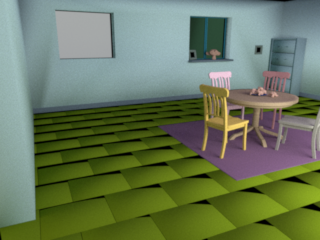
\includegraphics[width=\textwidth]{../FiguresDraft4/Figure3/Figure3_c.png}
        \label{fig:baseSceneTableChairs}
    \end{subfigure}
    
    \begin{subfigure}[b]{0.22 \textwidth}
        \caption{Indoor-plant}    
        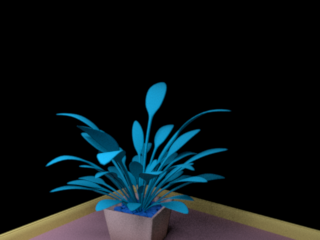
\includegraphics[width=\textwidth]{../FiguresDraft4/Figure3/Figure3_d.png}
        \label{fig:baseSceneIndoorPlant}
    \end{subfigure}    
    ~
    \begin{subfigure}[b]{0.22 \textwidth}
        \caption{Warehouse}    
        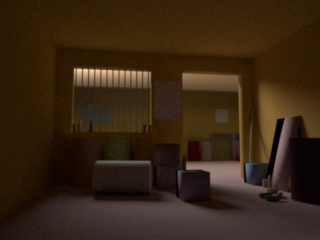
\includegraphics[width=\textwidth]{../FiguresDraft4/Figure3/Figure3_e.png}
        \label{fig:baseSceneWarehouse}
    \end{subfigure}
    ~
    \begin{subfigure}[b]{0.22 \textwidth}
        \caption{Checkerboard}    
        
\includegraphics[width=\textwidth]{../FiguresDraft4/Figure3/Figure3_f.png}
        \label{fig:baseSceneCheckerBoard}
    \end{subfigure}
    \caption{{\bf Example of base scenes form the VWCC library.} Each panel shows a rendering of one tamed base scene without additional objects inserted.  The reflectance spectra of the distinct surfaces in each scene has been assigned randomly (see below) using the VWCC software.  The light source spectra were also assigned randomly to the default and inserted light source.}\label{fig:baseScenes}
\end{figure}

\subsubsection{Virtual naturalistic scenes}

The light that reflects from objects to the eyes depends on many factors.
These include the surface reflectance, texture, material and geometry of the objects, the spectra of the illuminants, and the position of the observer.
We developed a rendering package (\href{https://github.com/BrainardLab/VirtualWorldColorConstancy}{Virtual World Color Constancy}, \href{http://rendertoolbox.org}{RenderToolbox4} \cite{heasly2014rendertoolbox3}) that allows us to construct models of naturalistic scenes, with key scene factors under programmatic control.
The package harnesses an open-source computer graphics renderer  \cite{jakob2015mitsuba} to produce physically-accurate images from the scene models.
Because each image is rendered from a known scene model, each image pixel can be labeled with the surface reflectance of the corresponding scene object.
By incorporating statistical models of the variation of object surface reflectance and daylight illumination, the pipeline allows us to produce large labeled sets of images that capture much of the task-relevant statistical structure of natural scenes.

% Figure 4
\begin{figure}
\centering
\begin{subfigure}[b]{0.14 \textwidth}
        \caption{Big-ball}
        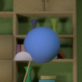
\includegraphics[width=\textwidth]{../FiguresDraft4/Figure4/Figure4_a.png}
        \label{fig:libraryWithBigBall}
    \end{subfigure}
    ~ 
\begin{subfigure}[b]{0.14 \textwidth}
        \caption{Small-ball}
        
\includegraphics[width=\textwidth]{../FiguresDraft4/Figure4/Figure4_b.png}
        \label{fig:libraryWithSmallBall}
    \end{subfigure}
    ~ 
    \begin{subfigure}[b]{0.14 \textwidth}
        \caption{Barrel}
        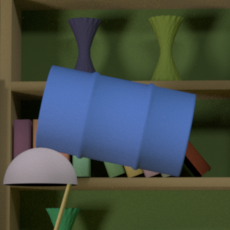
\includegraphics[width=\textwidth]{../FiguresDraft4/Figure4/Figure4_c.png}
        \label{fig:libraryWithBarrel}
    \end{subfigure}
    \begin{subfigure}[b]{0.14 \textwidth}
        \caption{Xylophone}
        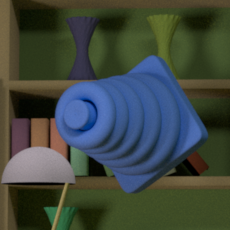
\includegraphics[width=\textwidth]{../FiguresDraft4/Figure4/Figure4_d.png}
        \label{fig:libraryWithXylophone}
    \end{subfigure}
    ~
	\begin{subfigure}[b]{0.14 \textwidth}
        \caption{Ring toy}
        
\includegraphics[width=\textwidth]{../FiguresDraft4/Figure4/Figure4_e.png}
        \label{fig:libraryWithRingToy}
    \end{subfigure}
        ~
    	\begin{subfigure}[b]{0.14 \textwidth}
        \caption{Bottle}
        
\includegraphics[width=\textwidth]{../FiguresDraft4/Figure4/Figure4_f.png}
        \label{fig:libraryWithChampagneBottle}
    \end{subfigure}
\caption{{\bf Library base scene with inserted objects.} The rendering package was used to insert different objects into the library base scene, with each panel showing a different object. The objects were inserted at a location in the image and then the camera was pointed at the object, so that the object's image is at the center of the rendered image.  In the figure panels, the full rendered image is cropped so that the inserted object is more visually salient. We use this capability of our software pipeline to insert target objects into scenes.}\label{fig:libraryWithTarget}
\end{figure}

Our rendering package includes a collection of base scenes (Fig.~\ref{fig:baseScenes}).
Base scenes specify an arrangement of objects and light sources.
Base scenes may be enriched by the insertion of additional objects, chosen from an object library (Fig.~\ref{fig:libraryWithTarget}).
Once the position, size and pose of the inserted objects has been set, our package allows the assignment of a surface reflectance function to each object in the scene and a spectral power distribution to each light source (Fig.~\ref{fig:VWCCTransformations}).
This provides a complete scene model which can be rendered from any specified viewpoint.

% Figure5
\begin{figure}
	\begin{subfigure}[b]{0.18 \textwidth}
    \centering
        \caption{Target position}
        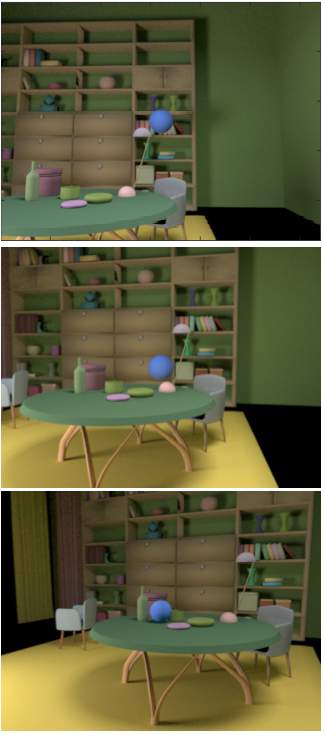
\includegraphics[width=\textwidth]{../FiguresDraft4/Figure5/Figure5_d.png}
        \label{fig:targetPositionVariation}
    \end{subfigure}
    ~
	\begin{subfigure}[b]{0.18 \textwidth}
    \centering
        \caption{Target size/Orientation}
        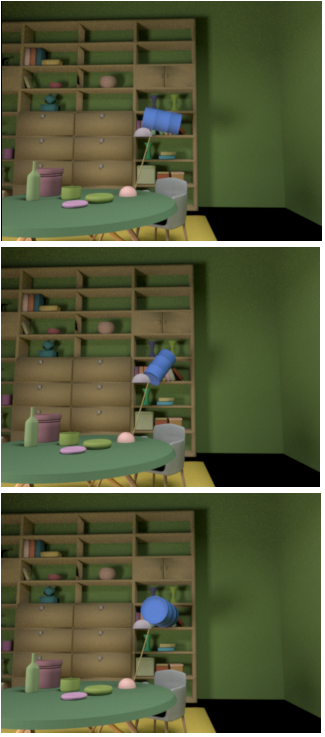
\includegraphics[width=\textwidth]{../FiguresDraft4/Figure5/Figure5_e.png}
        \label{fig:targetSizeOrientation}
    \end{subfigure}
~
\centering
	\begin{subfigure}[b]{0.18 \textwidth}
    \centering
        \caption{Target spectra}
        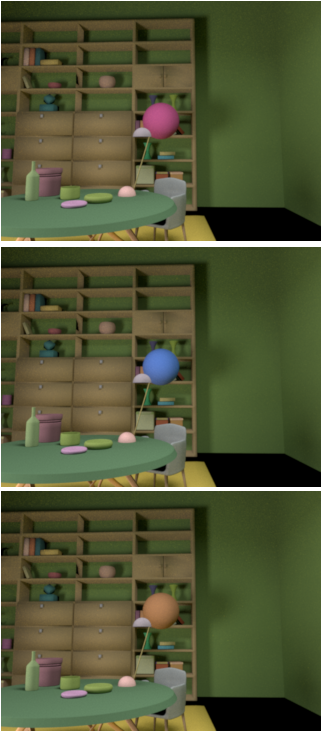
\includegraphics[width=\textwidth]{../FiguresDraft4/Figure5/Figure5_a.png}
        \label{fig:targetVariation}
    \end{subfigure}
    ~
    \begin{subfigure}[b]{0.18 \textwidth}
    \centering
        \caption{Background spectra}
        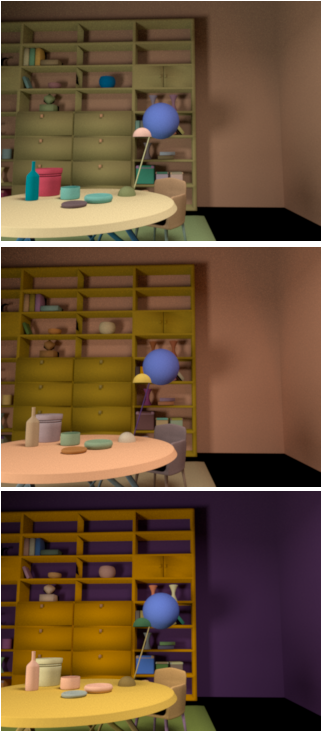
\includegraphics[width=\textwidth]{../FiguresDraft4/Figure5/Figure5_b.png}
        \label{fig:backGroundVariation}
    \end{subfigure}
    ~
    \begin{subfigure}[b]{0.18 \textwidth}
    \centering
        \caption{Illumination spectra}
        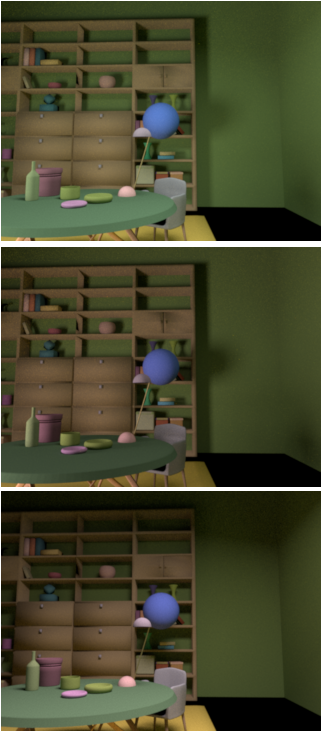
\includegraphics[width=\textwidth]{../FiguresDraft4/Figure5/Figure5_c.png}
        \label{fig:illuminationVariation}
    \end{subfigure}
    \caption{{\bf Transformations of the scene.} The possible transformations of the properties of a scene can broadly be classified into two groups: Geometrical (a-b) and Spectral (c-e). VWCC provides control over such transformation as illustrated by the columns. (a) The three panels in the column have the target object at three different positions. The camera points to the center of the pixel. (b) The target object in the three panels are at different orientations. (c) The target object surface reflectance varies across the three panels of the column. (d) The surface reflectance of the background objects varies across the three panels. In each panel, the reflectances were assigned randomly. (e) The power spectrum of the light sources were assigned randomly in the three panels. 
\label{fig:VWCCTransformations}}
\end{figure}

In the present work, we used our package to generate datasets of naturalistic scenes and corresponding images.
We used one fixed base scene and inserted a target object of fixed shape and size into this scene.
We generated three distinct datasets: Conditions 1-3.
Across these datasets the luminance constancy problem, estimating the target object LRV,
becomes progressively more difficult (Fig.~\ref{fig:studiedCases}).
Each dataset consisted of 1000 scenes and corresponding images.

%In Condition 0, the only source of stimulus variation was in the task relevant quantity, the target object LRV.
%Here, we fixed target object color (i.e. the relative reflectance spectrum of the target object),
%the reflectance spectra of the background objects, and the spectral power distributions of the light sources.
% Condition 0 defines a baseline. In this condition, all images with the same value of the LRV are identical.

In Condition 1, we only varied the surface reflectance spectrum of the target object.
The reflectance spectra of the background objects, and the spectral power distributions of the light sources were kept fixed.
In Condition 2, in addition to the reflectance spectrum of the target object,
we also varied the spectral power distribution of the light sources.
Finally, in Condition 3 we varied all three factors (target object surface 
reflectance spectrum, reflectance spectra of the background objects, 
spectral power distribution of the light sources).
We used 10 LRV values, equally spaced between 20 and 60 and generated 100 target surface reflectance spectra at these values. 
The surface reflectance spectra at the same LRV could differ in their relative shape.
The variation within our datasets captures the essence of the computational problem of lightness constancy
up to effects of scene geometry, an additional richness that we do not address in this paper.

% 1000 each Condition
%Condition 0: Baseline
%Condition 1: Target Color Only Variation
%Condition 2: Target Color and Background
%Condition 3: Target Color and Illuminant
%Condition 4a: Target Color, Background and Relative Illuminant
%Condition 4: Everything

For the primary results, we used the ``{\it Library}'' base scene and a spherical target object .
The library base scene contains X area lights. We inserted one additional spherical spherical light source into the scene.
The position and size of the inserted object, inserted light source and viewpoint were held fixed across all scenes in the database,
as shown in Figure~\ref{fig:3DScene}.
Surface and illuminant spectra were drawn according to statistical models of naturally occurring spectra.
We describe these models below.
Multispectral images ($320 \times 240$ pixels) were rendered at 31 evenly-spaced wavelengths between $400$nm and $700$nm.


%% Fix the title capitalization in a and b
\subsubsection{Illumination spectra}
% Figure 6
\begin{figure}
\centering
    \begin{subfigure}[b]{0.24 \textwidth}
    \centering
	\caption{Granada dataset}
        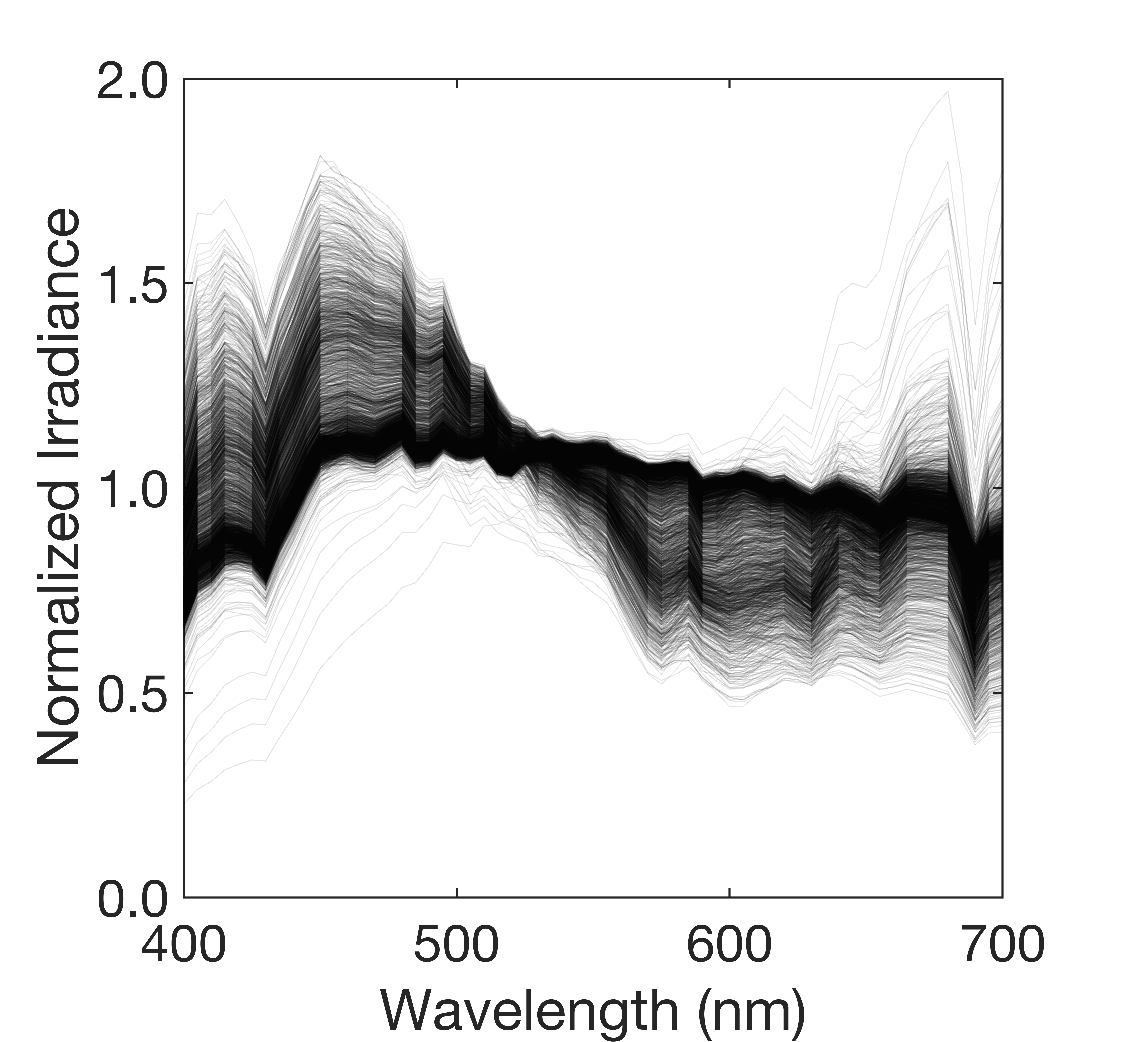
\includegraphics[width=\textwidth]{../FiguresDraft4/Figure6/Figure6_a.pdf}
        \label{fig:granadaData}
    \end{subfigure}
	\begin{subfigure}[b]{0.24 \textwidth}
    \centering
        \caption{Statistical model}
        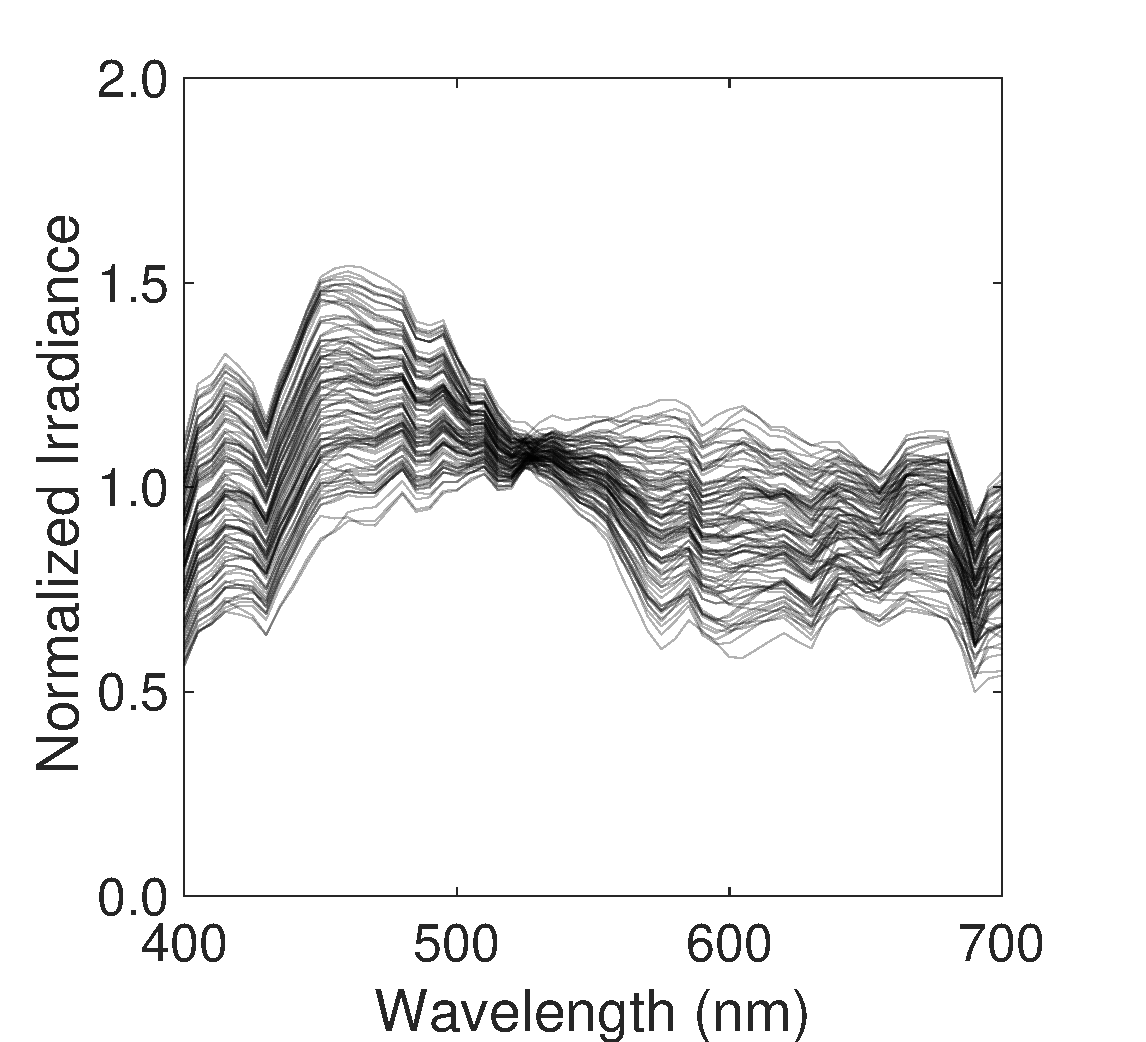
\includegraphics[width=\textwidth]{../FiguresDraft4/Figure6/Figure6_b.pdf}
        \label{fig:illuminantSamples}
    \end{subfigure}
      	\begin{subfigure}[b]{0.24 \textwidth}
    \centering
        \caption{CIE xy chromaticity}
        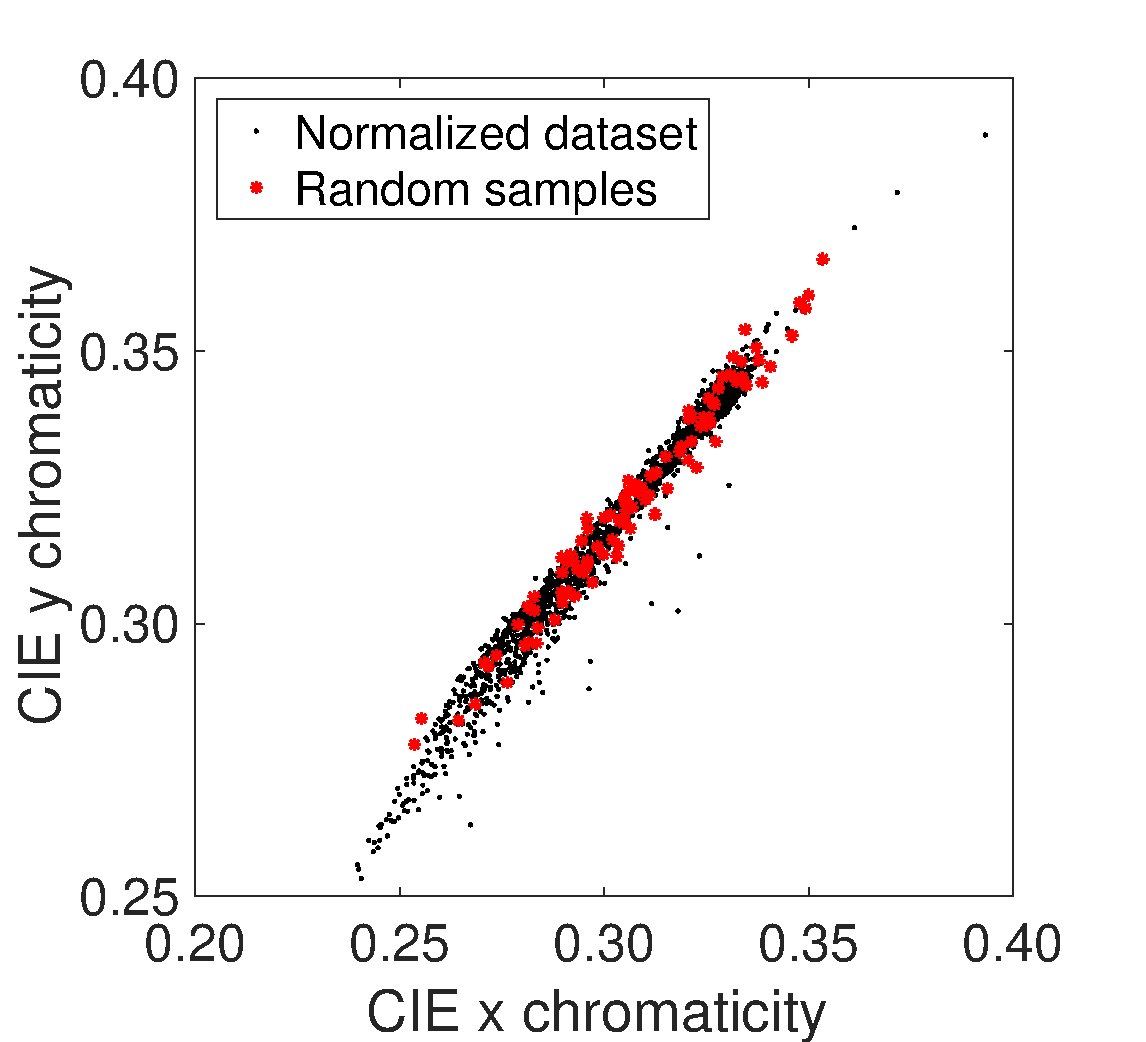
\includegraphics[width=\textwidth]{../FiguresDraft4/Figure6/Figure6_c.pdf}
        \label{fig:xyDiagram}
        \end{subfigure}
      	\begin{subfigure}[b]{0.24 \textwidth}
    \centering
        \caption{Color swatches}
        
\includegraphics[width=\textwidth]{../FiguresDraft4/Figure6/Figure6_d.pdf}
        \label{fig:sRGBIlluminant}
    \end{subfigure}
    \caption{{\bf Illumination spectra:} (a) Granada dataset. The spectra are normalized by the mean over wavelength. (b) A representative sample of spectra generated using normalized Granada dataset. (c) CIE xy chromaticity diagram of the normalized dataset and the random samples. (d) sRGB renditions of the samples from Figure~\ref{fig:illuminantSamples}.}
\label{fig:illuminant}
\end{figure}

To generate illumination spectra, we developed a statistical model of the \href{http://colorimaginglab.ugr.es/pages/Data}{Granada daylight measurements} \cite{hernandez2001color} and sample randomly from the model.
The overall intensity of the measurements spans approximately three orders of magnitude.
Figure~\ref{fig:granadaData} plots the measurements in normalized form to make apparent the variation in the relative spectra. The spectra are normalized by their mean over wavelength.

Our statistical model approximates these normalized shapes using their first 6 principle components, and models the variation in these components with
a 6-dimensional Gaussian whose mean and covariance matrix match the dataset's sample mean and covariance of the weights on these components \cite{BrainardFreeman}.
To generate a random relative illuminant spectrum, we take a draw from this Gaussian to obtain weights and generate the corresponding spectrum.
Figure~\ref{fig:illuminantSamples} illustrates the relative spectra of draws obtained using this procedure.
Details of the statistical model for illumination are provided in the appendix.

Because our multivariate Gaussian model is based on the rescaled spectra, it does not embody the large variation in overall intensity of natural daylights.
To obtain illuminant spectra with intensity variation similar to the Granada dataset, we scaled each randomly generated relative spectrum.
The scale factors we sampled at random in the range 0.15 and 150.
Color swatches of samples of illuminant spectra are shown in Figure~\ref{fig:sRGBIlluminant}.

\subsubsection{Surface reflectance spectra}
%% Fix the title capitalization in a and b
% Figure 7 Surface Reflectance Data and Model
\begin{figure}
\centering
	\begin{subfigure}{0.24 \textwidth}
    \centering
            \caption{Munsell and Vrhel dataset}
        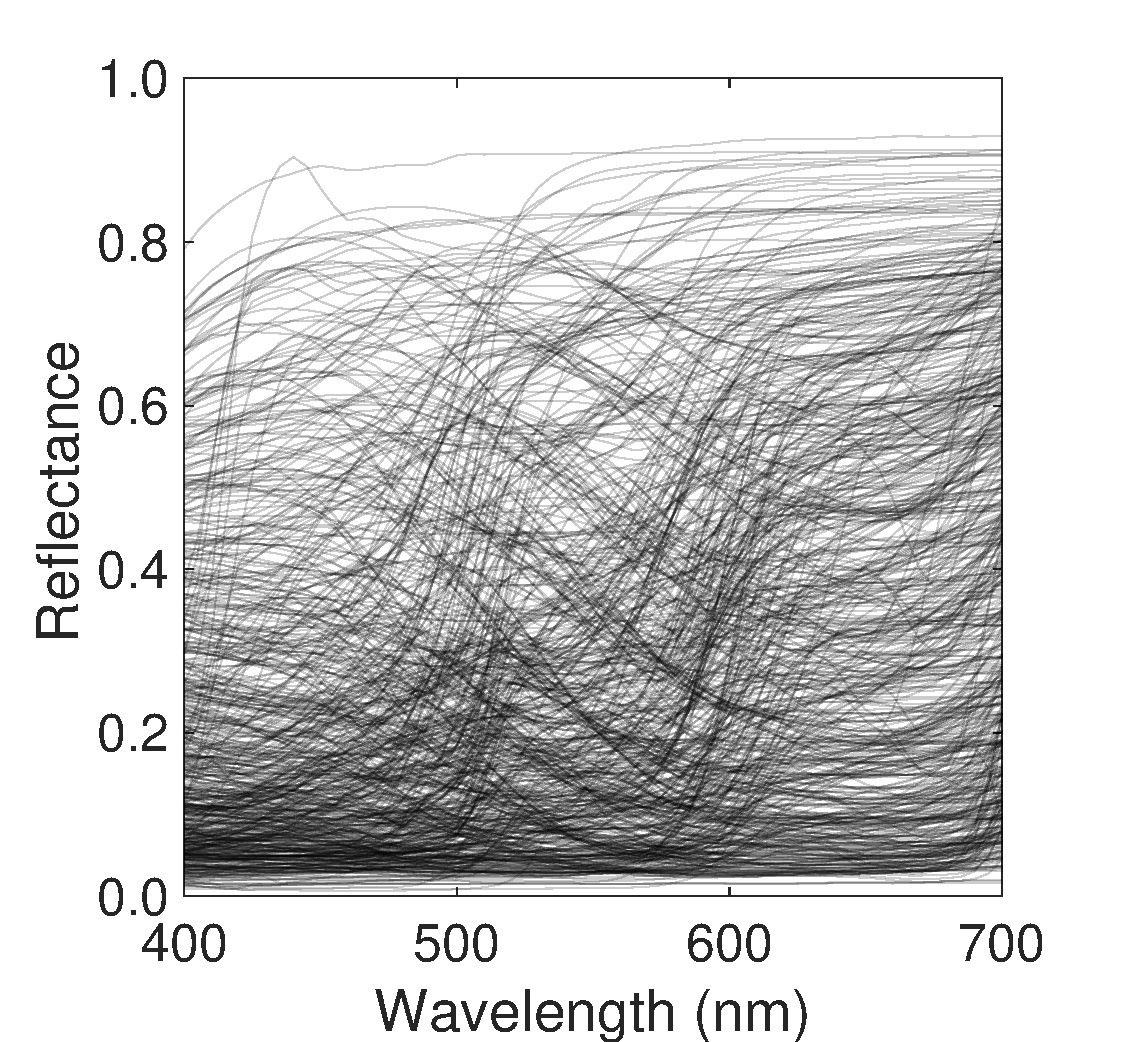
\includegraphics[width=\textwidth]{../FiguresDraft4/Figure7/Figure7_a.pdf}
        \label{fig:reflectanceSpectra}
    \end{subfigure}
    \begin{subfigure}{0.24 \textwidth}
    \centering
        \caption{Statistical model}
        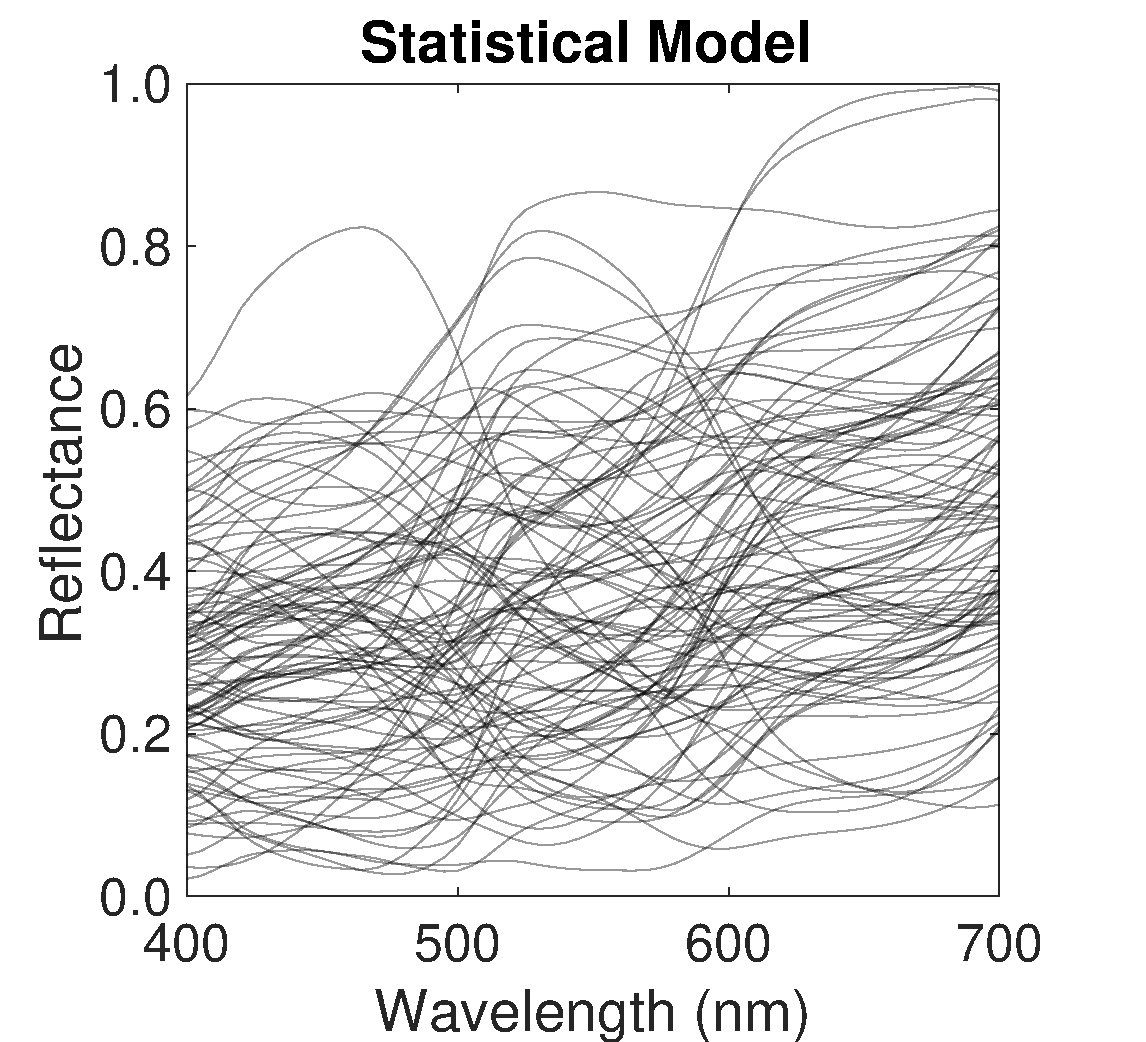
\includegraphics[width=\textwidth]{../FiguresDraft4/Figure7/Figure7_b.pdf}
        \label{fig:reflectanceSamples}
    \end{subfigure}
    \begin{subfigure}{0.24 \textwidth}
    \centering
    \caption{CIE xy chromaticity}
        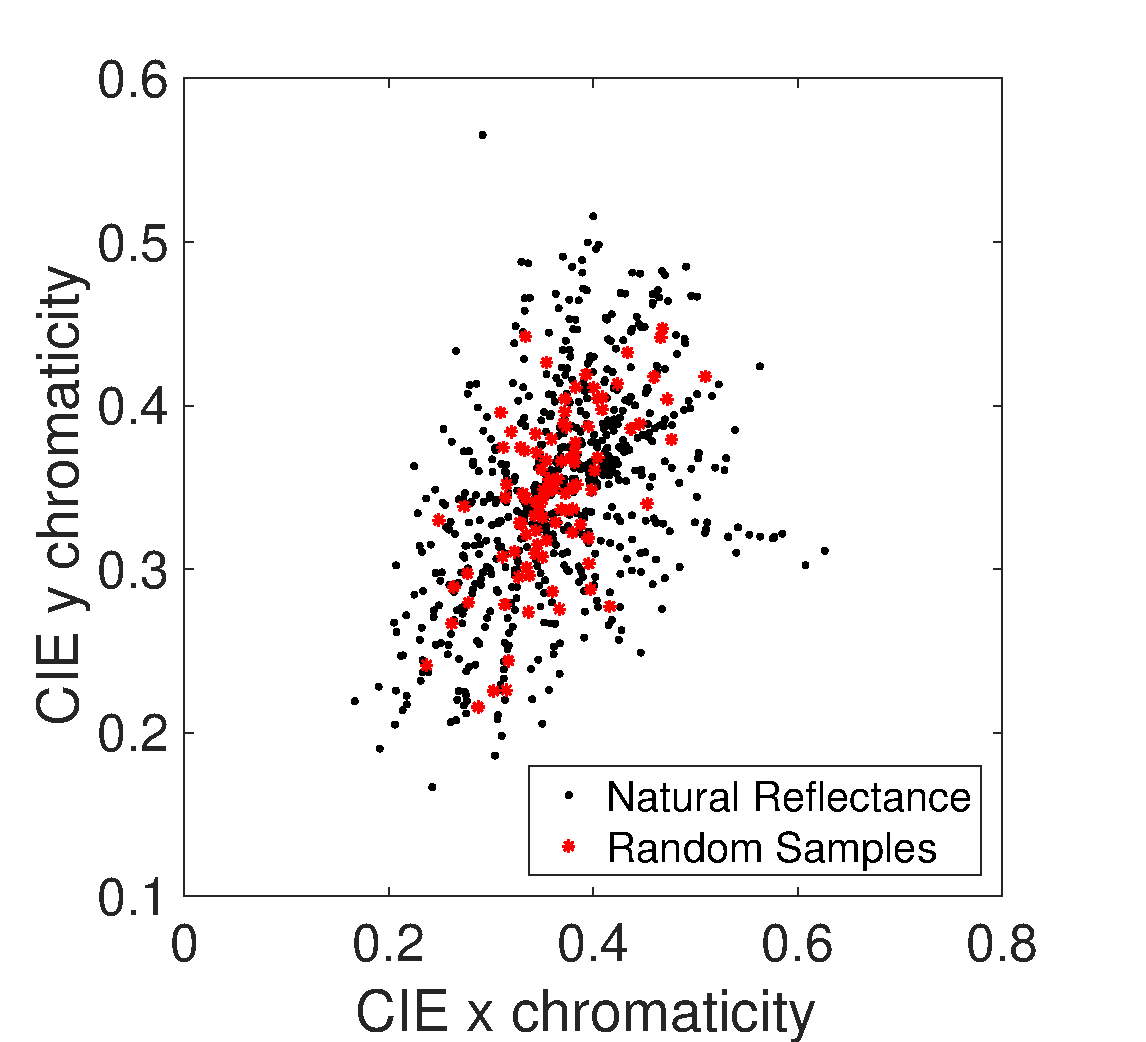
\includegraphics[width=\textwidth]{../FiguresDraft4/Figure7/Figure7_c.pdf}
        \label{fig:xyChroReflectance}
    \end{subfigure}    
    \centering
	\begin{subfigure}{0.24 \textwidth}
    \centering
        \caption{Color swatches}
        
\includegraphics[width=\textwidth]{../FiguresDraft4/Figure7/Figure7_d.pdf}
        \label{fig:backgroundSwatches}
    \end{subfigure}
    \caption{{\bf Surface reflectance spectra:} (a) Surface reflectance spectra from the Munsell and Vrhel datasets.(b) Representative samples of object surface reflectances. (c) CIE xy chromaticity diagram of the Munsell and Vrhel datasets (black) and samples of surface reflectances (red). (d) sRGB renditions of the samples of object surface reflectance under CIE D65 daylight.}
\label{fig:surfaceReflectanceGeneration}
\end{figure}

%Figure 8 Target Surface Reflectance Samples
\begin{figure}
\centering
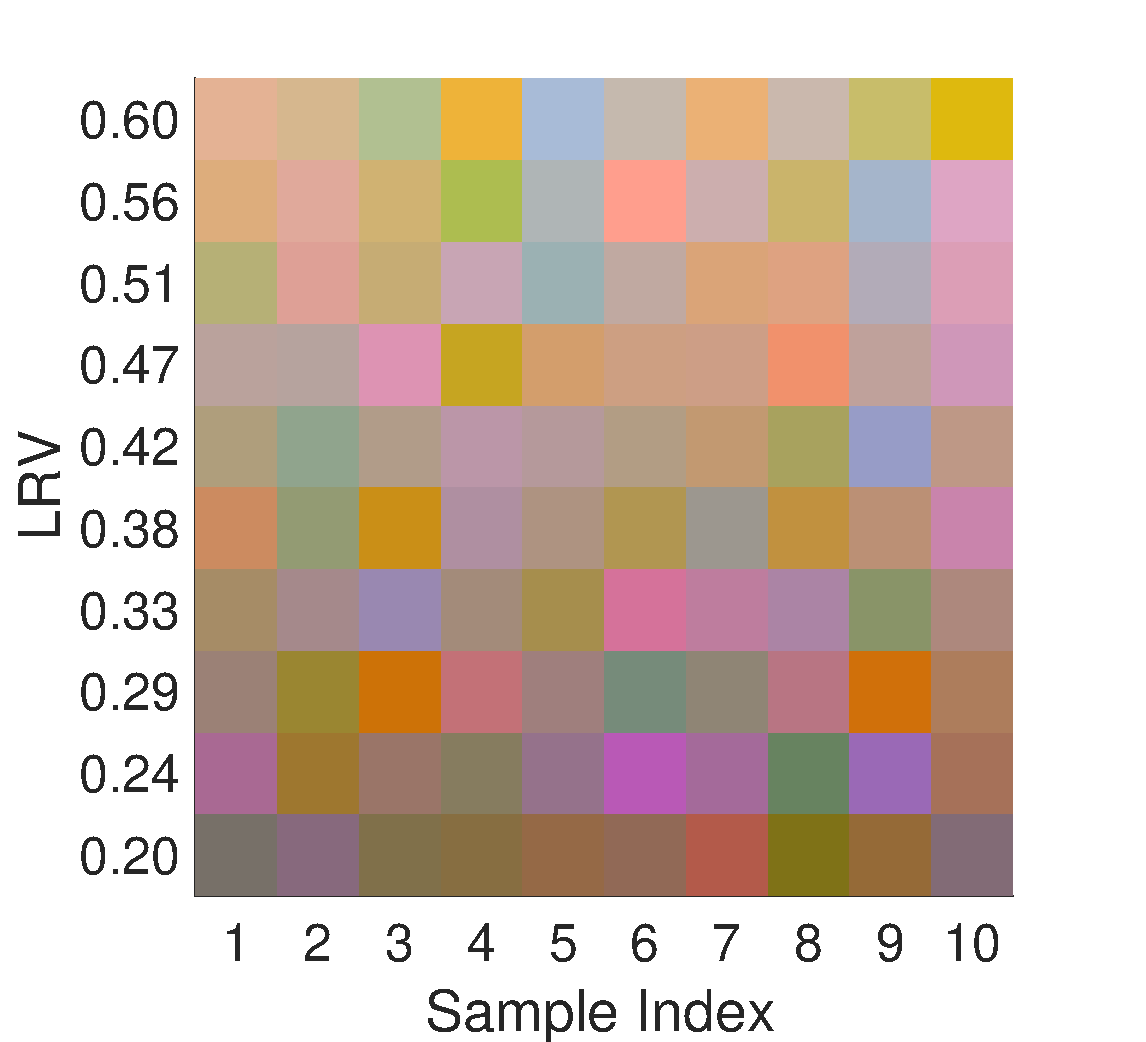
\includegraphics[width=0.3\textwidth]{../FiguresDraft4/Figure8/Figure8.pdf}
\caption{{\bf Target surface reflectance spectra:} sRGB renditions of the target object surface reflectance rendered under CIE D65 daylight spectrum. The figure shows 10 random samples at 10 equally spaced LRV levels in the range [0.2, 0.6]. This range captures more than 90\% of the natural surface reflectances. Each row contains 10 random samples of reflectance spectra generated at the LRV shown on the left.}
\label{fig:targetSwatches}
\end{figure}


We generated random reflectance spectra using the same principles we applied to generate random illuminant spectra.
We combined the Munsell \cite{kelly1943tristimulus} and Vrhel \cite{vrhel1994measurement} surface reflectance 
measurements to create a database containing 632 reflectance spectra Figure~\ref{fig:reflectanceSpectra}.
The Munsell database contains 462 spectra each measured at 5nm sampling intervals between 380nm and 780nm.
The Vrhel dataset contains 170 spectra measured at 2nm sampling between 390nm and 730 nm.
We resampled these spectra to 31 evenly-spaced wavelengths between $400$nm and $700$nm.
Figure~\ref{fig:reflectanceSpectra} illustrates the spectra of draws obtained using this procedure.
Details of the statistical model for surface reflectance spectra are provided in the appendix. 

For generating the target object reflectance at a particular luminance $(Y_{\rm T})$, the values in a generated spectrum were 
scaled such that the LRV had the desired value (see appendix).
Figure \ref{fig:targetSwatches} shows color swatches of target reflectance spectra rendered under CIE illuminant D65, for evenly spaced LRV values.

% Figure 8: Methods
\begin{figure}
\centering
\begin{subfigure}[b]{0.25 \textwidth}
		\centering
        \caption{sRGB rendering of a 3D scene}
        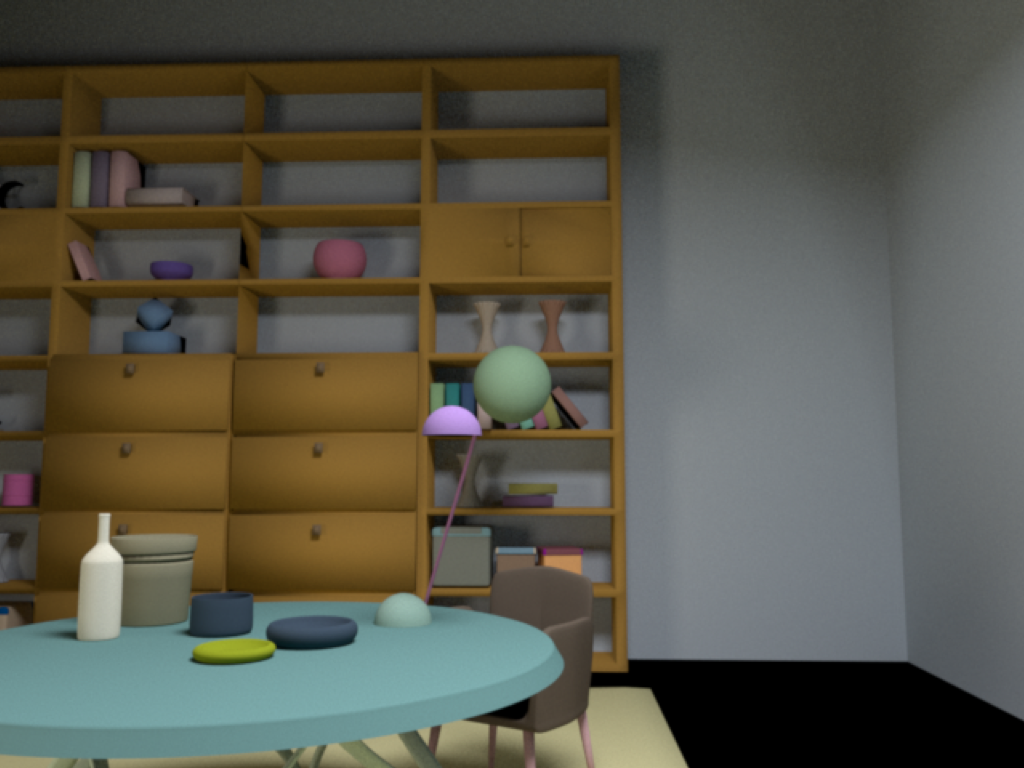
\includegraphics[width=\textwidth]{../FiguresDraft4/Figure9/Figure9_a.png}
        \label{fig:3DScene}
    \end{subfigure}
    ~ 
    \begin{subfigure}[b]{0.19 \textwidth}   
    \hspace{0.1 \textwidth}
        \caption{Cropped image}
        \vspace{1.5mm}
        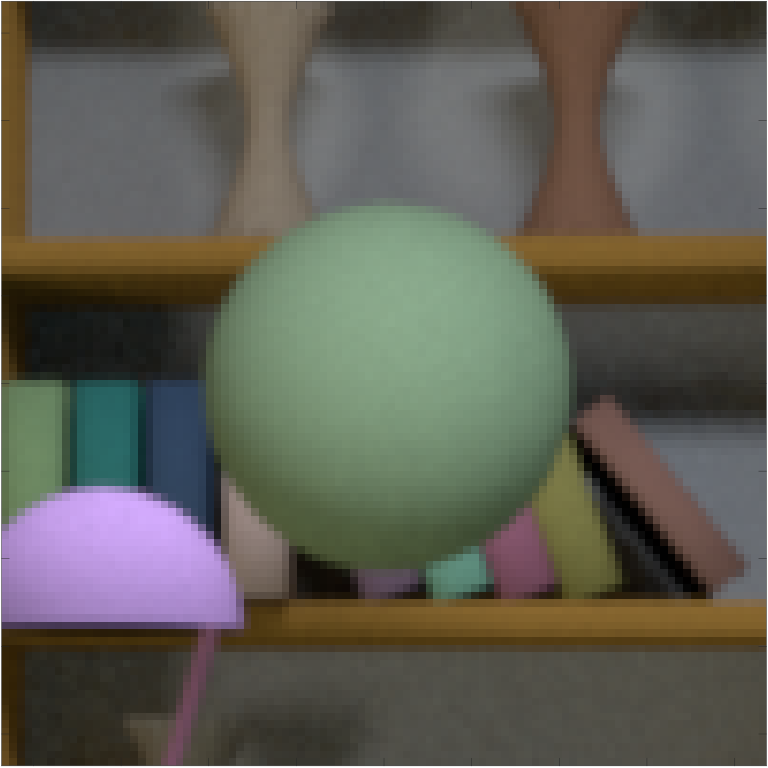
\includegraphics[width=\textwidth]{../FiguresDraft4/Figure9/Figure9_b.png}
        \label{fig:croppedImage}
    \end{subfigure}
    ~ 
    \begin{subfigure}[b]{0.19 \textwidth}
    \hspace{0.1 \textwidth}
        \caption{Optical image}
        \vspace{1.5mm}
        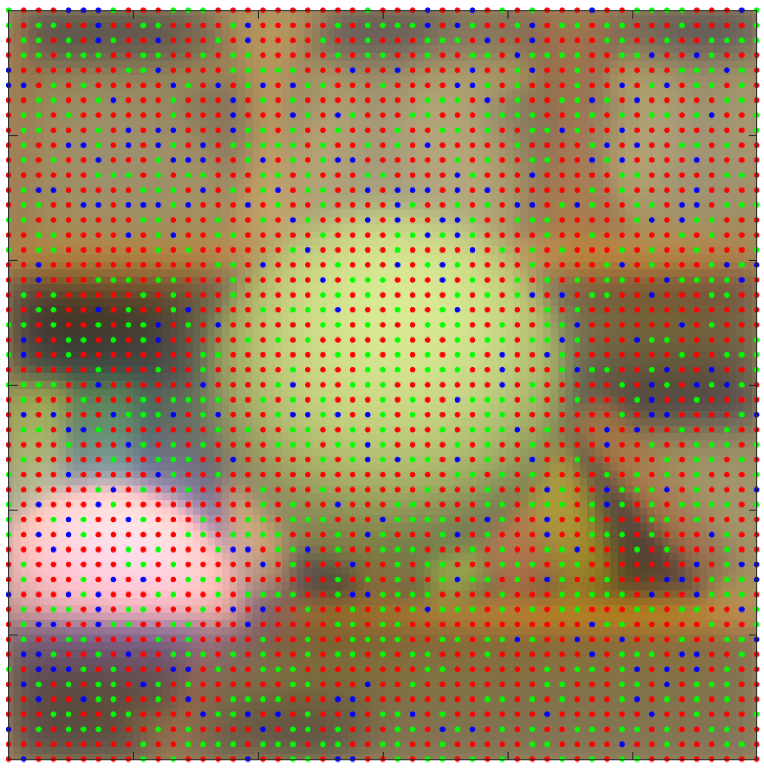
\includegraphics[width=\textwidth]{../FiguresDraft4/Figure9/Figure9_c.png}
        \label{fig:croppedImageWithMosaic}
    \end{subfigure}
    ~
    \begin{subfigure}[b]{0.2 \textwidth}
        \caption{LMS cone contrast}
        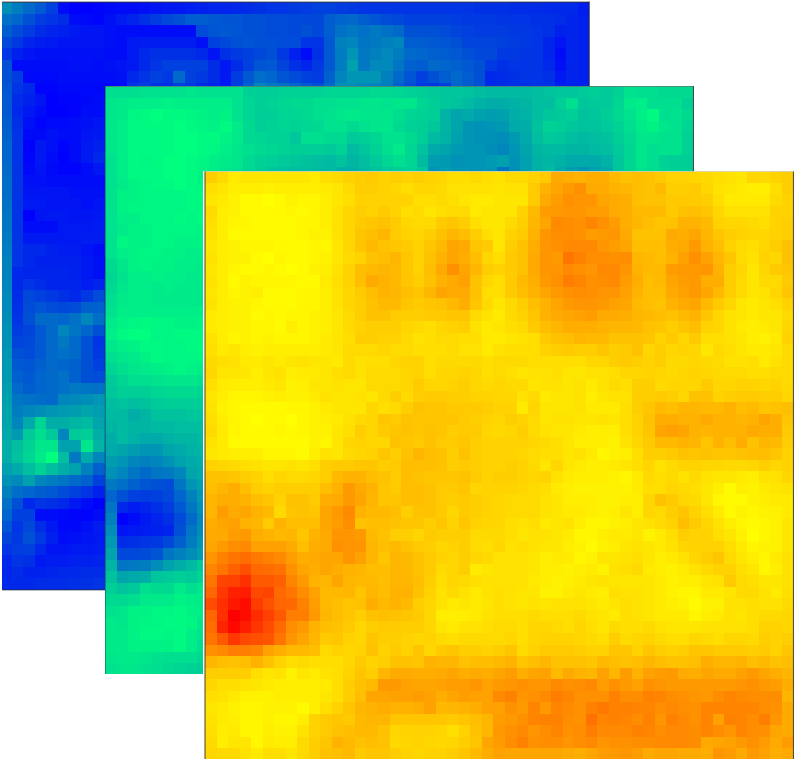
\includegraphics[width=\textwidth]{../FiguresDraft4/Figure9/Figure9_d.png}
        \label{fig:coneContrast}
    \end{subfigure}
    \label{fig:sceneWithCroppedImage}
    \caption{{\bf Generating labeled dataset for computational analysis:}  For the supervised approach employed in this work, the labeled database is generated as follows: (a) A 3D virtual scene, containing a target object of known surface luminance is created. The target object is placed in the camera field of view. After assigning spectra to the light sources and other other objects in the scene, a multispectral image of the scene is rendered using the Mitsuba software package. (b) The central portion of the rendered image, which contains the target object, is cropped from the image. (c) The retinal image incident on the cone mosaic after optical blurring and the location and the identity of the cones (L cones: Red, M cones: Green, S cones: Blue).  (d) The cone responses are interpolated to estimate the responses of all the three types of cone at each location (demosaicing). Finally, the demosaiced images are contrast normalized separately for each cone type.}
\end{figure}

\subsection{Model of early visual system} \label{method:Isetbio}

The light entering the eye is blurred by the eye's optics.
The resulting retinal image is sampled by a mosaic of cone photoreceptors.
The responses of these photoreceptors provide the information about the scene that is available to the neural visual system for further processing.
Because we are interested in how well luminance constancy may be achieved by the human visual system, we simulated the cone responses
to our scenes using a model of the early visual system.

We focussed our analysis on regions of the image local to the target by cropping the rendered images to $1 \times 1$ degrees of visual angle around the target object ($51 \times 51$ pixels; Figure~\ref{fig:croppedImage}).
This choice is motivated by the observation that neural receptive fields early in the visual pathways (e.g., retina, primary visual cortex) pool information locally.
In foveal primary visual cortex, receptive fields have a spatial extent of approximately 1 degree of visual angle (REFS).
% Johannes to provide his favorite citation or two.  Some review.

We modeled a visual system with a pupil diameter of 3 mm, optical blurring (including axial chromatic aberration) in the formation of the retinal image (REF whatever optics model), spatial sampling by an interleaved mosaic of long (L), middle (M)  and short (S) wavelength-sensitive cones (Brainard mosaic review; Fig.~\ref{fig:croppedImageWithMosaic}). The cone mosaic contained  L:M:S cones in the ratio 0.6:0.3:0.1 and with spectral sensitivities derived from the CIE physiological standard (REF).
Cone isomerizations were computed assuming an integration time of 5 msec, and we modeled the Poisson nature of photopigment isomerization (REF Hecht et al). This modeling was implemented using the software infrastructure provided by ISETBio (REF).

% Details from Nicolas (TEXT IN CAPS IS FROM VIJAY)
% Scene: 
%- the default mean luminance was set to 200, but there is a key-value param that could have overriden this value. 
%  I do not know if this were the case.
%
% % MEAN LUMINANCE = 0, NO SCALING

%- The default FOV was 1 deg, but there is a key-value param that could have overriden this value.
%  I do not know if this were the case.
%
% % HORIZONTAL FOV = 1

%- Distance default is 1 meter, but there is  a key-value param that could have overriden this value.
%  I do not know if this were the case.
%
%% DISTANCE 1M

%
%Optics: 
%- 3 mm pupil, 17 mm focal length, with a spectro-spatial OTF described in  
%  (Marimont & Wandell (1994) J. Opt. Soc. Amer. A,  v. 11, p. 3113-3122), 
%   which includes axial chromatic aberration. However, there is key-value param o skip the OTF. 
%   Not sure if this was used.  It it was used, the optics was set to diffraction limited.
%
% % SKIP OTF OFF:  'skipOTF', false ...  

%
%Lens: 
%- not sure if the optical density is from Wyszecki&Stiles or from Stockman-Sharpe. 
%  The isetbio file commend only says it is from PTB. David do you know, or should I check
%  the data?
%
%Cone Mosaic: 
%- rectangular cone mosaic with 0.6:0.3:0.1 LMS densities
%- FOV was a key-value param, so I do not know what was used.
%- Also the mosaic was subsampled  according to a cone-stride param, with a default of 15 cones
%but there is a key-value param that could have overriden this value. I do not know what that parameter value was.
%
% CONE STRIDE = 3 'coneStride', 3, ... 

%
%- There is a key-value pair to also low-pass the optical image with default value to not do so.
%  If that was user-overriden the OI was lowpass filtered using a Gaussian whose sigma was dependent on the cone-stride param.
%
% LOW PASS FILTER = MATCH CONE STRIDE : lowPassFilter = 'matchConeStride';      

%- IntegrationTime was not specified, so it was the default which is 5 msec.
%  The cone isomerization maps were also demosaiced using linear interpolation.
%- The default isomerization noise was set to none, but there is a key-value parameter
%  that can override it. I do not know what the value of that was.
%
% ISOMERIZATION NOISE = FROZEN, 'isomerizationNoise', 'frozen'

%-  Finally, there is a key-value param named 'coneEfficiencyBasedReponseScaling', which by default is set to 'none'
%   But if it was user-set to non 'none' the code scaled the responses to simulate equal quantal efficiencies 
%   for L , M and S coneEfficiencyBasedReponseScaling by undoing filtering by the lens and the macular pigment.
%   I do not know if this was used.
% 
% coneEfficiencyBasedReponseScaling = 'area'


The cone isomerizations represent the first step of visual processing.
To capture key properties of post-receptoral processing, such as contrast normalization \cite{heeger1992normalization,albrecht1991motion,carandini2012normalization},
we processed the isomerizations as follows:
First, we generated a response for each cone class at each pixel in the sampled retinal image, using bilinear interpolation separately for each cone class.
This gives us a cone response image for each cone class.
We also normalized each cone response image by the total area under the corresponding cone spectral sensitivity.
This makes the magnitude of the cone response images similar across cone classes.
These two processing steps do not alter the information in the cone response images. 

To model contrast coding, we converted each cone response image to a corresponding cone contrast image.
This was accomplished by computing the mean response over the three cone contrast images, and then subtracting off and dividing by this mean.
To model contrast normalization, we divided by the sum of squared contrasts over image pixels and cone classes.

\subsection{Computational luminance constancy} \label{method:SupervisedLearning}
We used our datasets to determine how well target object LRV can be estimated from cone responses and from normalized cone contrasts.
Studying both representations allows us to understand how early contrast coding and normalization affect how well luminance constancy can be achieved.
We applied accuracy maximization analysis (AMA) to learn the optimal receptive fields for estimating LRV,
and evaluated the performance obtained when the output of these filters was optimally decoded.

\subsubsection*{Learning optimal filters}
AMA is a task specific Bayesian method for dimensionality reduction.
When provided with a labeled training set, a receptive field response model, a decoder that uses these responses to estimate the stimulus label, and a cost function, AMA returns a set of linear receptive fields.
Given a set of linear receptive fields and an explicit cost function, it is possible to determine the minimum-expected-cost estimator that maps responses to stimulus labels given the training set and the 
assumption that all images in the training set are equally likely.
Moreover, the corresponding expected estimation cost may be explicitly computed.
AMA searches over the space of linear receptive fields to find the set that minimizes the expected estimation cost.
Here we used squared error as the cost function and assumed that receptive field responses were corrupted by scaled Gaussian noise (i.e. Poisson-like noise with a fano factor of 1.3).
Details of how AMA learns filters and the filter responses are optimally decoded are provided in previously published work \cite{geisler2009optimal,burge2017accuracy,jaini2017linking}.

\subsubsection*{Decoding optimal filters}

Once the optimal receptive fields have been learned, we need to develop a general decoder that can be applied to arbitrary test stimuli.
A general decoder is necessary because the decoder used to learn the receptive fields requires the response mean and response variance of the filters to every labelled stimulus in the training set \cite{geisler2009optimal,burge2017accuracy}.
To proceed, first we use the AMA optimal receptive fields and the training dataset to find the conditional distributions of the receptive field responses, conditioned on the labelled target object LRVs.
Then, we approximate these with multivariate Gaussian distributions.
With the Gaussian approximation in hand, 
to estimate the LRV of the target object in a test image, we use Bayes' rule to obtain the posterior distribution over LRV values given the filter responses.
The optimal estimate is the LRV value that minimizes the expected value of the cost function, where the expectation is taken over the posterior.

\subsubsection*{Baseline methods}

To provide baselines for evaluation of the estimation method described above, we used linear regression.
First, we solved for the weights on the average L, M and S cone responses target object that best predicted the target LRV values.
We took the average cone respones from a $3 \times 3$ region at the center of the target object.
This baseline method disregards information carried the image regions corresponding to the background objects.
We also performed regression on the contrast normalized version of the cone responses.
This baseline method indirectly incorporates information carried the image regions corresponding to the background objects,
through their effect on the contrast normalized responses from the target object. 
We also evaluated the performance of a naive model that estimate the mean of the LRV values in the training set, irrespective
of the image data.

\section{Results} \label{Results}
%% Figure 10: Results for Condition 1
\begin{figure}
\centering
            \begin{subfigure}[b]{0.25 \textwidth}
        \caption{LRV estimates}
        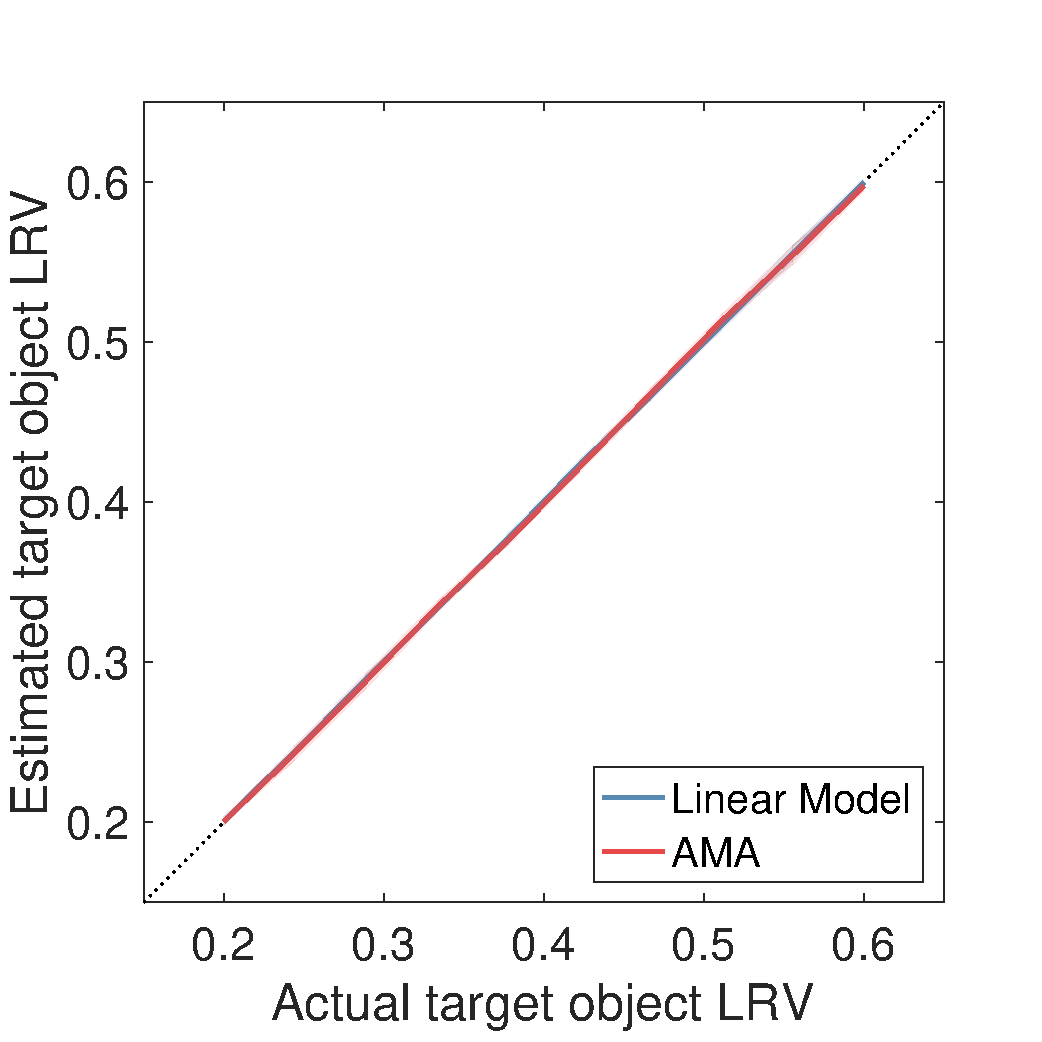
\includegraphics[width=\textwidth, trim={0 0 0 1.3cm},clip]{../FiguresDraft4/Figure10/Figure10_a.pdf}
        \label{fig:case1Estimates}
    \end{subfigure} 
        \begin{subfigure}[b]{0.26 \textwidth}
        \caption{Receptive field response}
        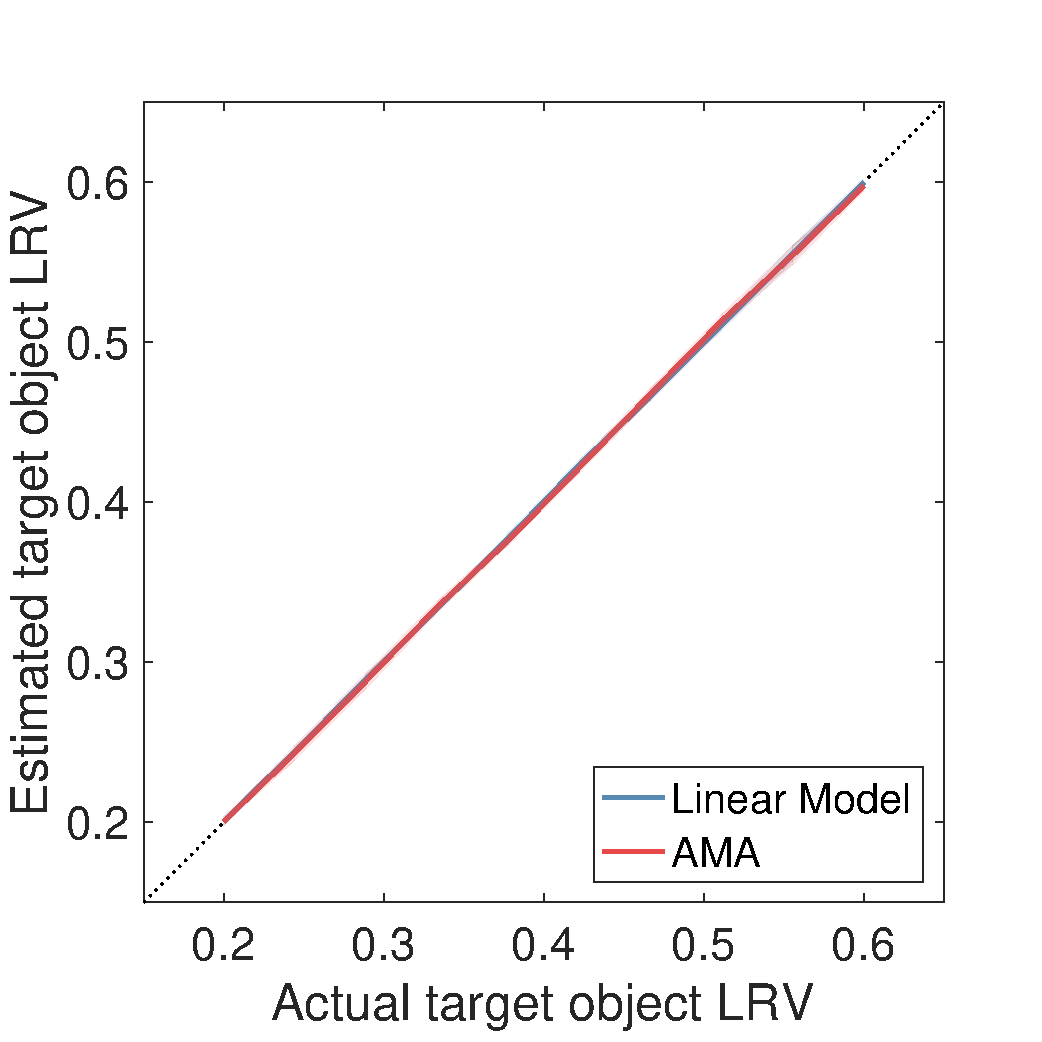
\includegraphics[width=\textwidth, trim={0 3mm 0 15mm},clip]{../FiguresDraft4/Figure10/Figure10_b.pdf}
        \label{fig:case1RFResponse}
    \end{subfigure}
    ~
    \begin{subfigure}[b]{0.28 \textwidth}
	\caption{AMA receptive fields}
	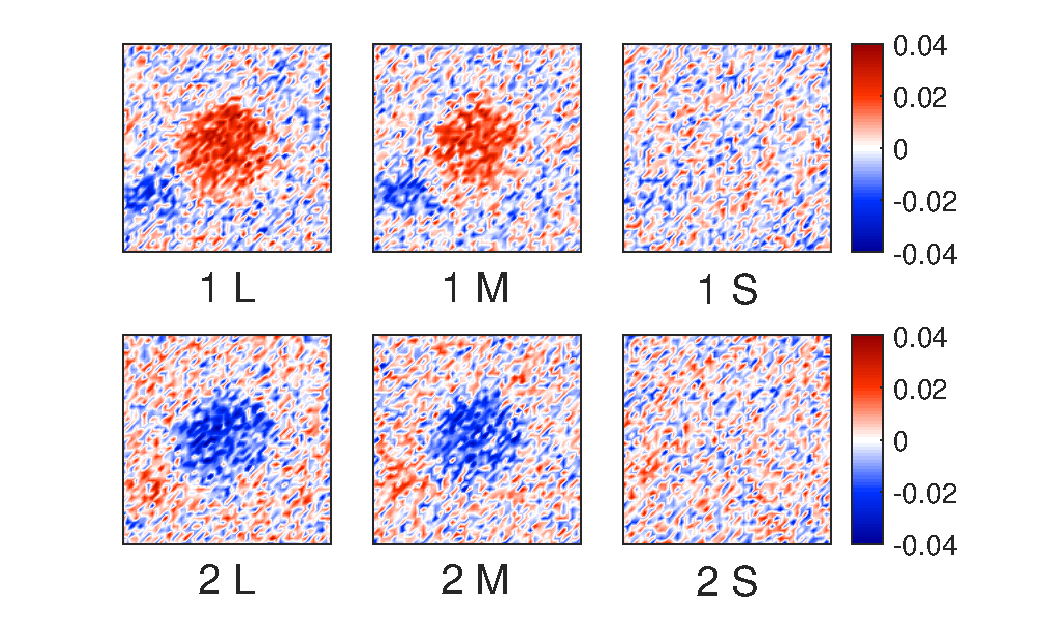
\includegraphics[width=1.07\textwidth, trim={0 -0.6cm 0 -0.3cm}]{../FiguresDraft4/Figure10/Figure10_c.pdf}
	\label{fig:case1RFs}
    \end{subfigure}   
    \caption{{\bf RF response and luminance estimates for condition 1:} (a) Photoreceptor response projected along the first two AMA receptive fields for images of condition 1. We show the response for the images in the training set. Each response cloud represents the response of images corresponding to one LRV. The response clouds are approximated by a multivariate Gaussian whose mean and variance are approximated by the ellipses shown in the figure. (b)  Estimated v/s assigned target LRV for the image in condition 1. Solid lines show the mean estimate, the filled region in light color shows $\pm$ 1 standard deviation. Relative error of estimation is 0.8\% (Linear regression) and 1.1\% (AMA) . The diagonal unit slope (blue dotted) line is for reference. The standard deviations are too small to be visible.}
\label{fig:Condition1}
\end{figure}

We start with Condition 1, where only the LRV and relative reflectance spectrum of the target object vary across scenes.
For this condition, estimating LRV should be easy because the variation in target object reflectance that we introduced
preserved LRV (which is calculated using a CIE D65 as the illumination).
This in turn means that for fixed scene illuminants similar to D65, the luminance of the light reflected from the target object will vary minimally.
In Condition 1, we used an illumination draw form our daylight sample and thus expect a reasonable degree of similarity to D65.

We used AMA to learn a set of linear receptive fields that are optimal for estimating target LRV for this condition.
For this condition, we trained and evaluated AMA on the cone responses to the image patches.
Figure~\ref{fig:case1RFResponse} shows the responses of the first two receptive fields to all the image patches in the training set.
Each individual point represents the receptive field responses to a single image patch.
Each point is color coded according to the LRV corresponding to the target object in the patch.
The responses segregate according to the target LRV.
This means that the responses may be used to accurately decode LRV, confirming the intuition that computational
luminance constancy is readily achieved for Condition 1.

Decoding performance for the test set is shown in Figure~\ref{fig:case1Estimates}.
As expected, the LRV estimates obtained by decoding the AMA receptive field responses are veridical.
Figure~\ref{fig:case1Estimates} also shows the performance of the baseline linear regression method, again trained
on the training set and evaluated on the test set.
For this condition, linear regression on the target object cone responses also leads to veridical LRV estimates.

Figure~\ref{fig:case1RFs} shows the first two AMA receptive fields.
Each of these, in essence, takes a weighted sum of the L and M cone isomerizations at the target object location.
The isomerizations in the background regions and the S cone isomerizations are largely ignored.
These receptive fields make sense.
For this condition, the background regions provide very little task relevant information: their only relevant effect is
through light scattered from them onto the target.
In addition, luminance is primarily determined by L and M cone isomerizations.

%% Figure condition 2: Isomerization Fails
\begin{figure}
\centering
    \begin{subfigure}[b]{0.22\textwidth}   
        \caption{RF response (Isomerization)}
        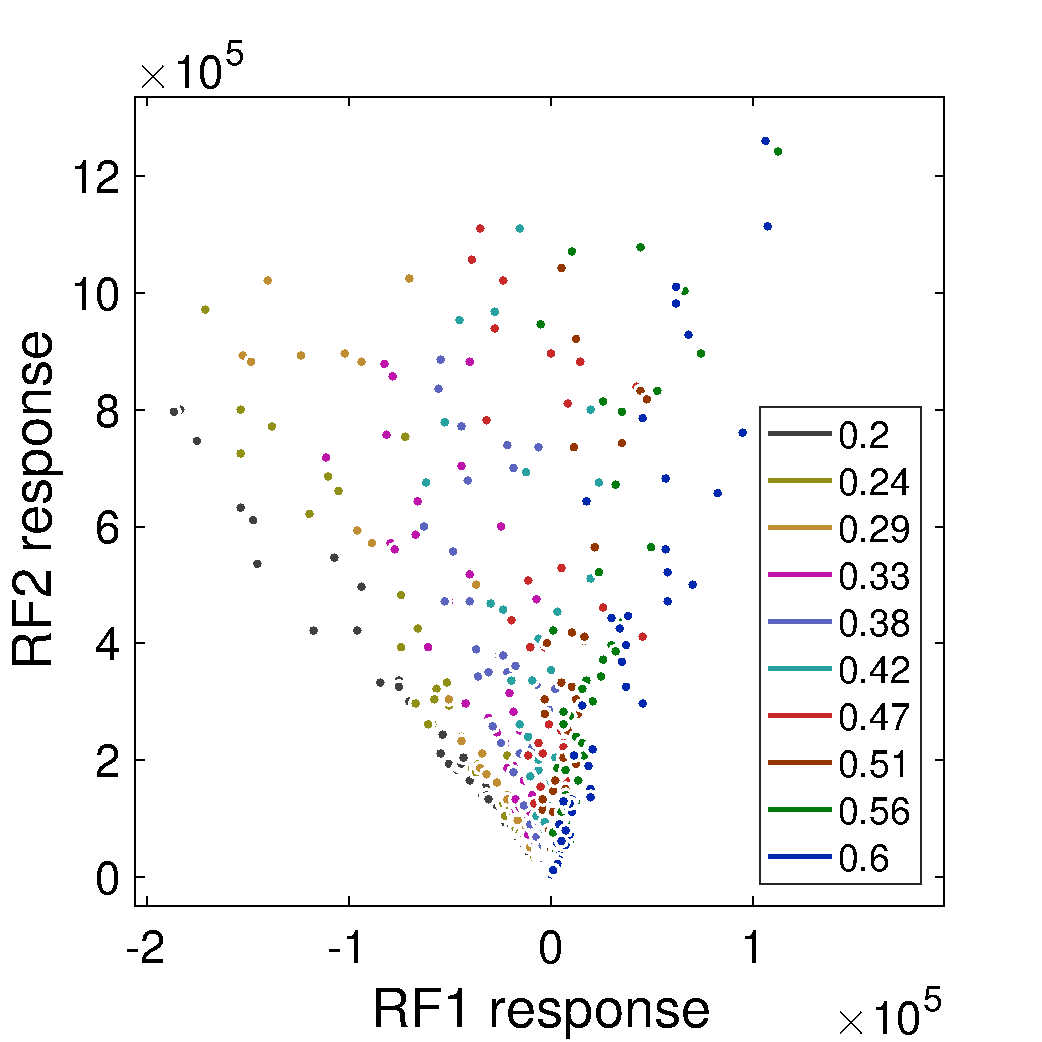
\includegraphics[width=\textwidth]{../FiguresDraft4/Figure11/Figure11_a.pdf}
        \label{fig:case2IsomerizationEstimates}
    \end{subfigure}
        \begin{subfigure}[b]{0.22 \textwidth}
        \caption{LRV estimates (Isomerization)}
        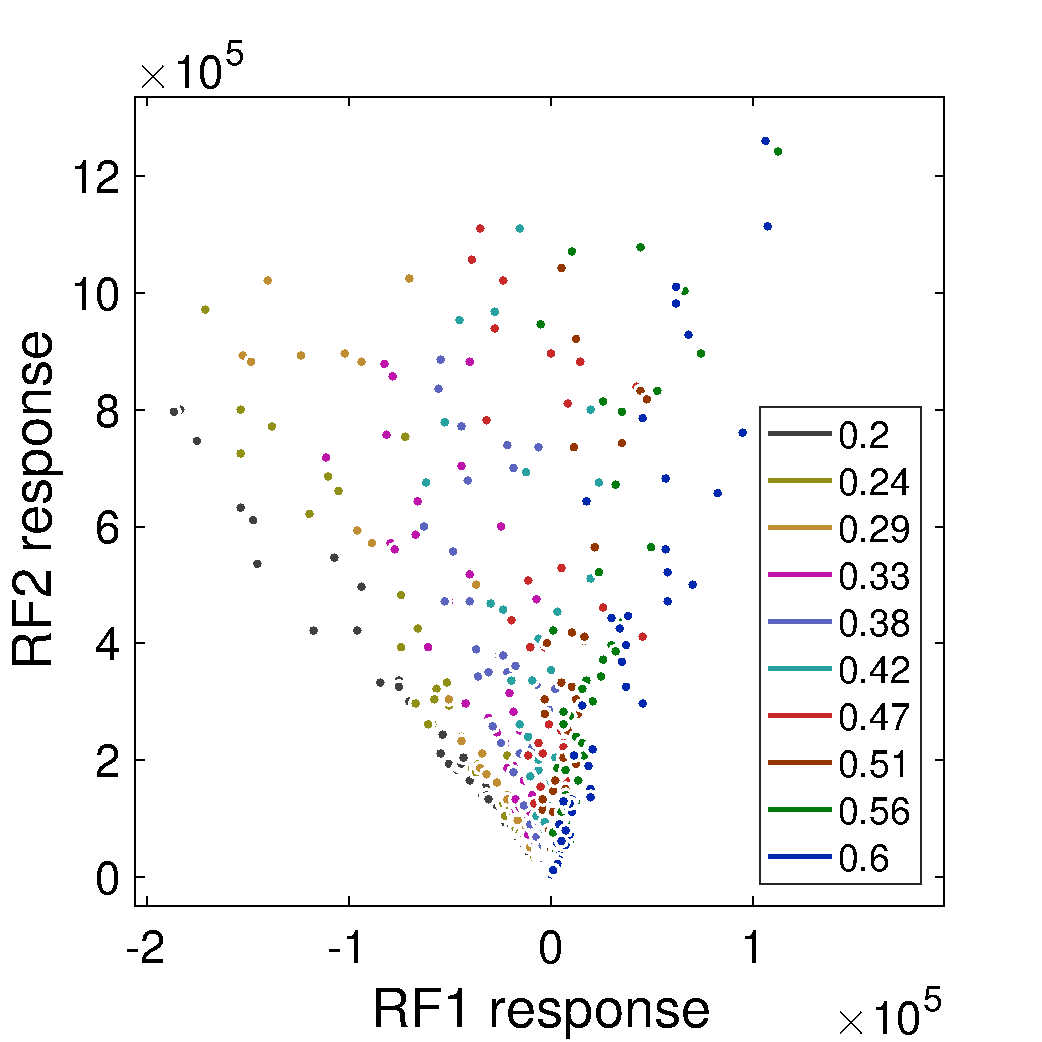
\includegraphics[width=\textwidth]{../FiguresDraft4/Figure11/Figure11_b.pdf}
        \label{fig:case2RFResponseIsomer}
    \end{subfigure}
            \begin{subfigure}[b]{0.22 \textwidth}
        \caption{RF response (Contrast)}
        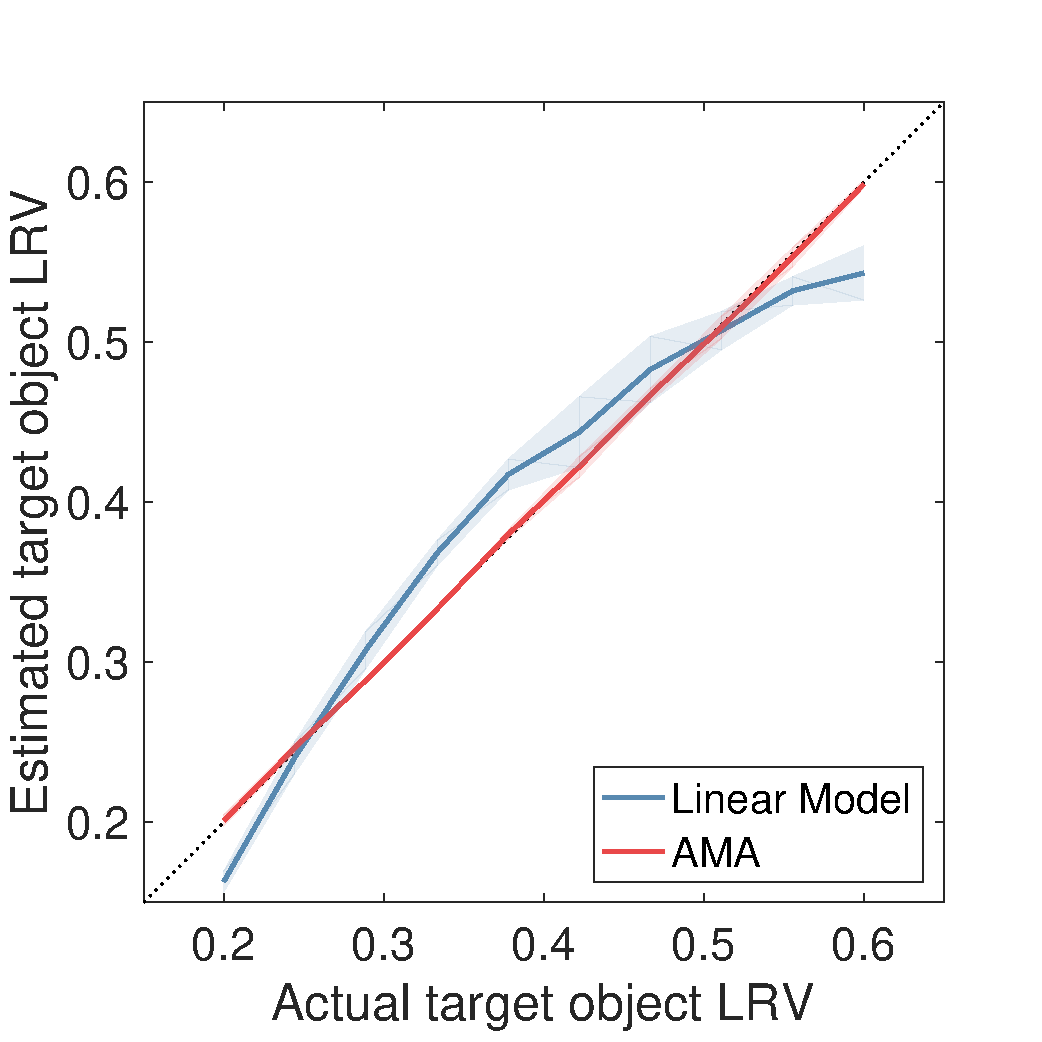
\includegraphics[width=\textwidth]{../FiguresDraft4/Figure11/Figure11_c.pdf}
        \label{fig:case2ContrastEstimates}
    \end{subfigure}
            \begin{subfigure}[b]{0.22 \textwidth}
        \caption{LRV estimates (Contrast)}
        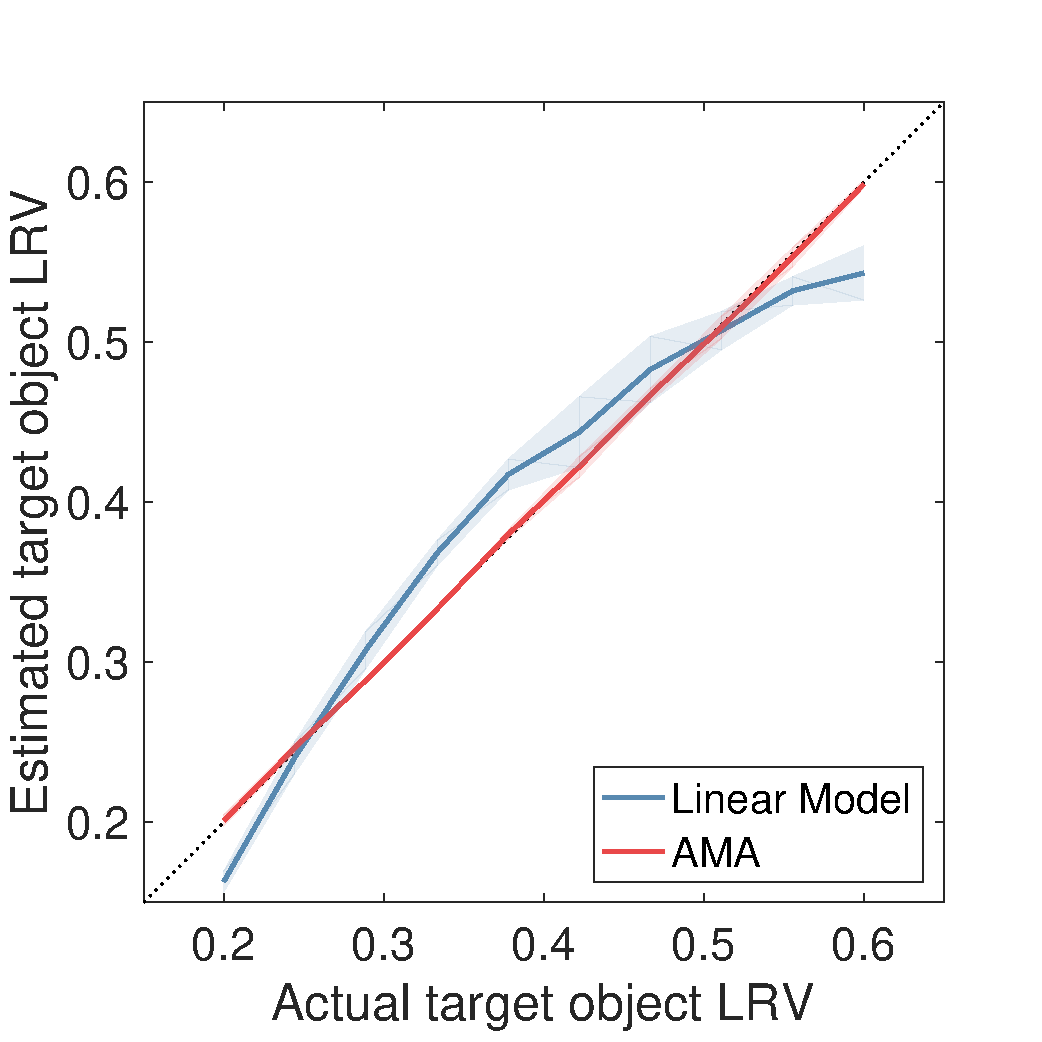
\includegraphics[width=\textwidth]{../FiguresDraft4/Figure11/Figure11_d.pdf}
        \label{fig:case2RFResponseContrast}
    \end{subfigure}
    \caption{{\bf Condition 2: Luminance can be estimated using the contrast signal:} (a) Photoreceptor response projected on AMA receptive fields calculated using photoreceptor response. (b) Mean LRV $\pm$ 1 standard deviation for images in the test set obtained using linear regression and AMA. The relative error of estimation is 41.4\% (Linear regression) and 31.3\% (AMA). (c) The contrast normalized photoreceptor response projected along the first two AMA receptive fields. The receptive fields were calculated using the contrast normalized stimuli. The response at each luminance level separates much better in this representation. (d) Estimated v/s assigned target LRV for the image in condition 2. The relative error of estimation is 9.3\% (Linear regression) and 1.1\% (AMA).}
\label{fig:Condition2}
\end{figure}

Next we discuss Condition 2, where we introduce variation in the spectral power distribution function of the light sources.
This variation makes the task more difficult, because it causes more variation in cone isomerizations due to factors other than the target object LRV.
Figure~\ref{fig:Condition2}(a, b) show the results when we learned and evaluated the performance of AMA on the cone isomerizations.
Performance is poor.
Indeed, on average the estimates track deviate considerably from the true LRV, as seen by the fact that the mean estimate
(red line) does not lie along the positive diagonal and by the fact that there is large estimation variability for each
value of the true LRV (as indicated by the width of the shaded red region).
For this case, linear regression is also very poor. Indeed, the linear regression estimates are essentially the same as would be obtained
by simply guessing the mean LRV of the training set (0.4).

Recall that there are two qualitatively distinct aspects to the variation in light source spectra.
One is a variation in relative spectral power distribution and the
other is a variation in overall intensity.
To separate the effect of these two aspects, we trained and evaluated AMA on the contrast normalized cone isomerizations.
Figure~\ref{fig:Condition2}(c, d)shows that performance improves greatly, and indeed is essentially perfect.
This observation is consistent with a large literature on computational color constancy that shows that when only illumination spectra are varied,
contrast-based representations provide an effective vehicle for achieving color constancy (REFS).
That same literature, however, shows that
contrast-based representations are less effective at supporting constancy when the spectra of background objects in the scene vary.

%% Figure 12: Results for Condition 3
\begin{figure}
\centering
            \begin{subfigure}[b]{0.25 \textwidth}
        \caption{LRV estimates}
        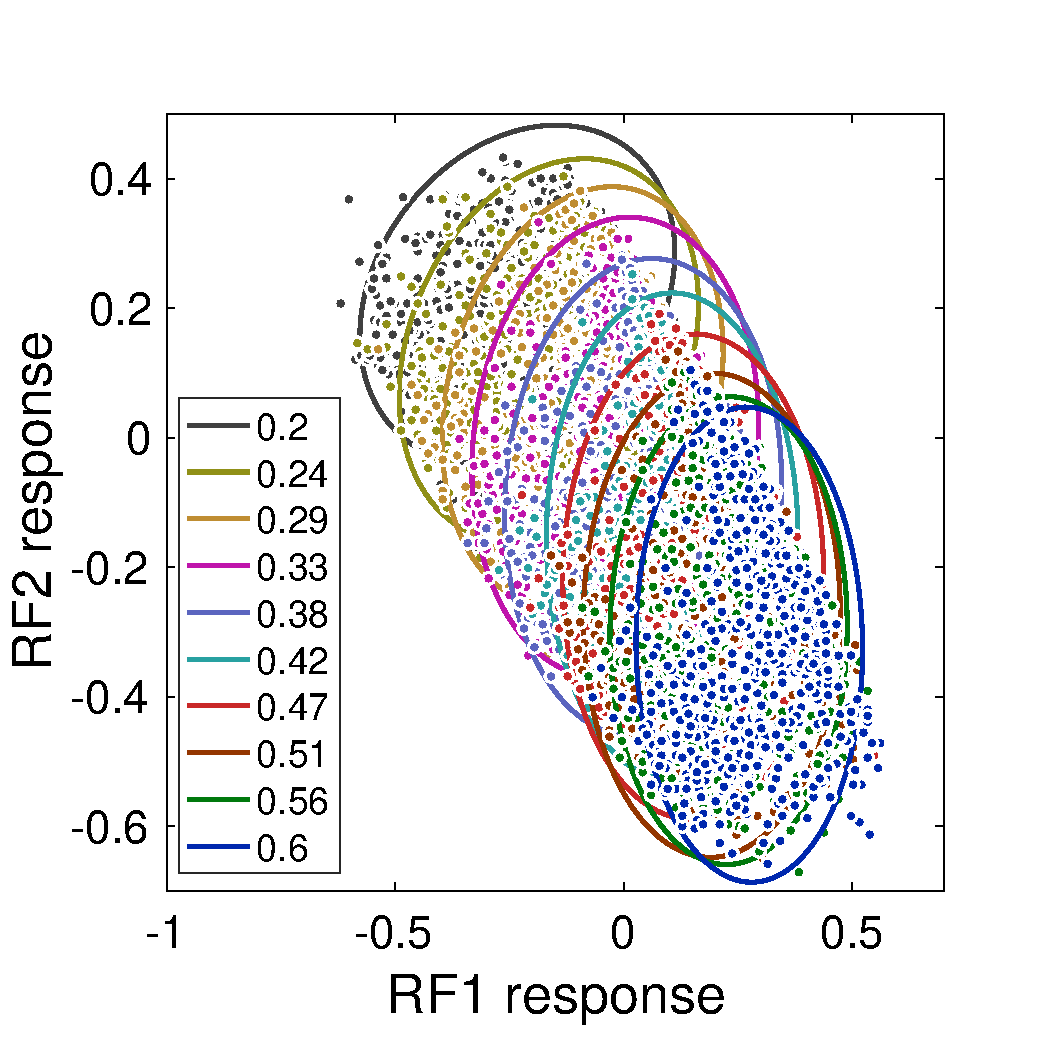
\includegraphics[width=\textwidth, trim={0 0 0 1.3cm},clip]{../FiguresDraft4/Figure12/Figure12_a.pdf}
        \label{fig:case3Estimates}
    \end{subfigure} 
        \begin{subfigure}[b]{0.26\textwidth}
        \caption{Receptive field response}
        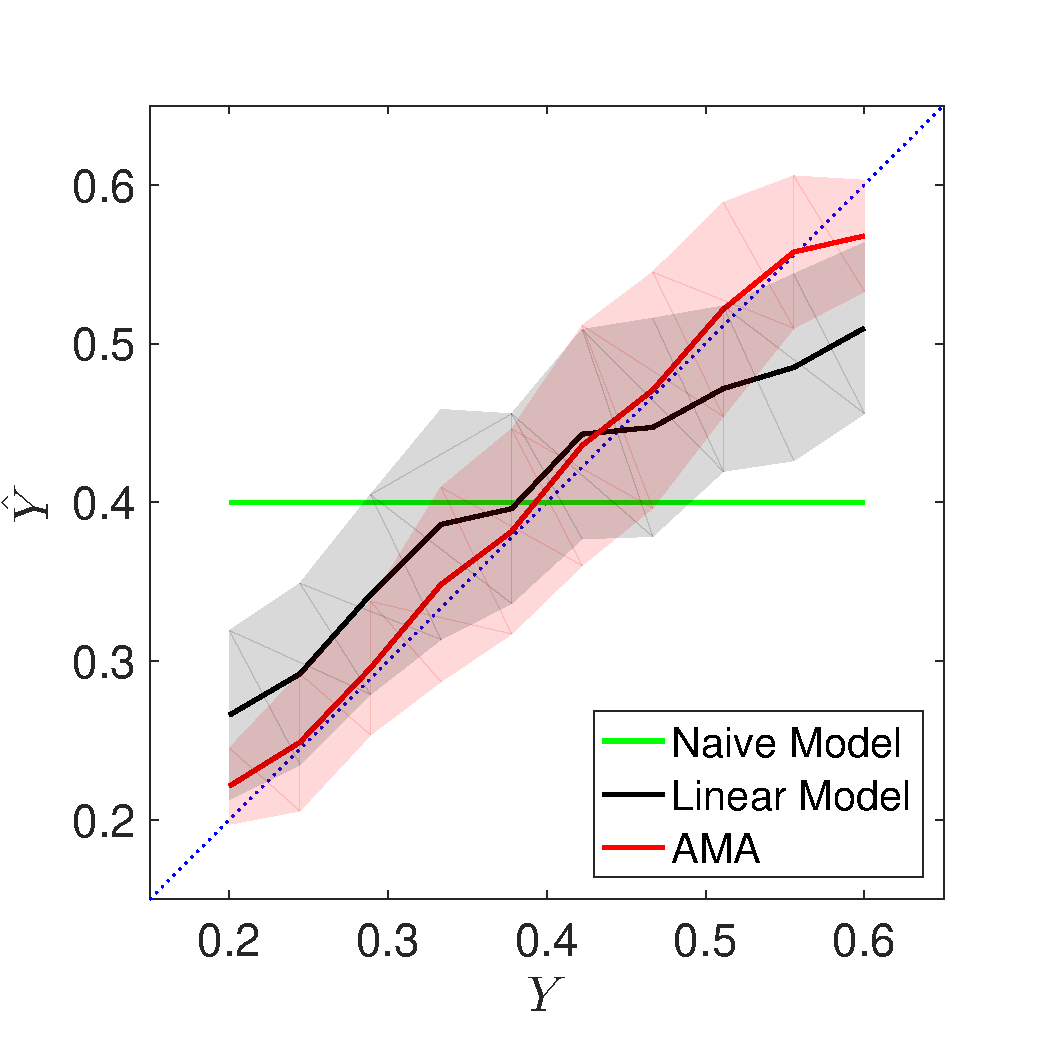
\includegraphics[width=\textwidth, trim={0 3mm 0 15mm},clip]{../FiguresDraft4/Figure12/Figure12_b.pdf}
        \label{fig:case3RFResponse}
    \end{subfigure}
    ~
    \begin{subfigure}[b]{0.28 \textwidth}
	\caption{AMA receptive fields}
	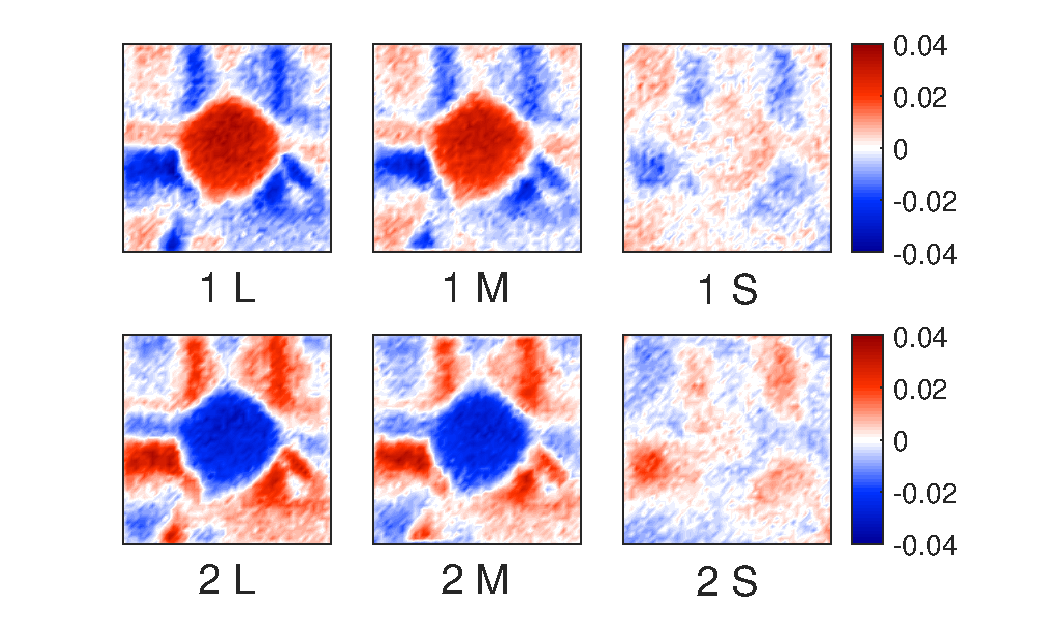
\includegraphics[width=1.07\textwidth, trim={0 -0.6cm 0 -0.5cm}]{../FiguresDraft4/Figure12/Figure12_c.pdf}
	\label{fig:case3RFs}
    \end{subfigure}       \caption{{\bf RF response and luminance estimates for condition 3:} (a) Photoreceptor response projected along the first two AMA receptive fields for images of condition 1. We show the response for the images in the training set. Each response cloud represents the response of images corresponding to one LRV. The response clouds are approximated by a multivariate Gaussian whose mean and variance are approximated by the ellipses shown in the figure. (b)  Estimated v/s assigned target LRV for the image in condition 1. Solid lines show the mean estimate, the filled region in light color shows $\pm$ 1 standard deviation. The relative error of estimation is 22.9\%  for linear regression and 13.0\% for AMA. The diagonal unit slope (blue dotted) line is for reference. The standard deviations are too small to be visible.}
\label{fig:Condition3}
\end{figure}

In Condition 3, we introduced variation in the reflectance spectra of the background objects.
This condition models the full real-world spectral variation that is most relevant for the computational problem of luminance constancy.
We again trained and evaluated AMA for labeled images patches in this condition using the contrast-normalized cone isomerizations.
Figure~\ref{fig:case3Estimates} shows the results.
The LRV estimates obtained via AMA are more variable and less accurate than for the previous conditions.
None-the-less, the estimates provide useful information about the target LRV.
Indeed, on average the estimates track the true LRV, as seen by the fact that the mean estimate
(red line) tracks the positive diagonal.
The increased estimation variability is indicated by the width of the shaded red region.
Performance of baseline linear regression method (also for the contrast normalized isomerizations) is worse than that of the AMA-based estimates.

Figure~\ref{fig:case3RFResponse} shows the responses of the first two AMA linear receptive fields for test [or training] stimuli.
Here, there is considerable overlap in the receptive field responses for stimuli having different LRV values.
Recall, however, that performance is based on six rather than two receptive fields.
Inclusion of more receptive fields reduces the ambiguity visible in the responses of just the first two.

Figure~\ref{fig:barGraphs} summarizes luminance constancy performance across the conditions, for both AMA and linear regression. 
We quantified overall performance in terms of overall relative root mean squared estimation error (relative RMSE) for the test set defined as:
\begin{align}
E_{\rm rel} = \sqrt{\left\langle\left(\frac{\rm{LRV_{Estimated}-LRV_{True}}}{\rm{LRV_{True}}}\right)^2\right\rangle}
\label{eq:relRMSe}
\end{align}
where the expectation is taken over all test stimuli at all LRVs.
The height of each bar gives the relative RMSE for each method and condition.
Note first that AMA improves upon linear regression for all conditions but the first, where performance for both methods is essentially perfect.
This is expected since AMA makes optimal use of the stimulus information under a wider range
of conditions than linear regression.
Moreover, the linear regression method we use as a baseline here
only has access to cone isomerizations at image locations corresponding to the target object, while AMA has access to isomerizations from the entire image patch.
Second, the fact that performance for Condition 2 is very poor tells us that that when there is substantial intensity variation in the illuminant, achieving luminance constancy
directly from the cone isomerizations is difficult.
Performance improves greatly when we consider the same condition but when the cone isomerizations are contrast normalized. 
Indeed, AMA performance for this case is, as in Condition 1, essentially perfect.
Note, however, that Condition 2 does not include variation in the background surface reflectances.
Such reflectances vary scene to scene in natural viewing.
The results for Condition 3 show performance when we add such variation into the training and test sets.
The error here represents the overall level of luminance constancy that our methods achieve for the
most realistic condition that we tested.

% Figure Error Bar Graphs
\begin{figure}
\centering
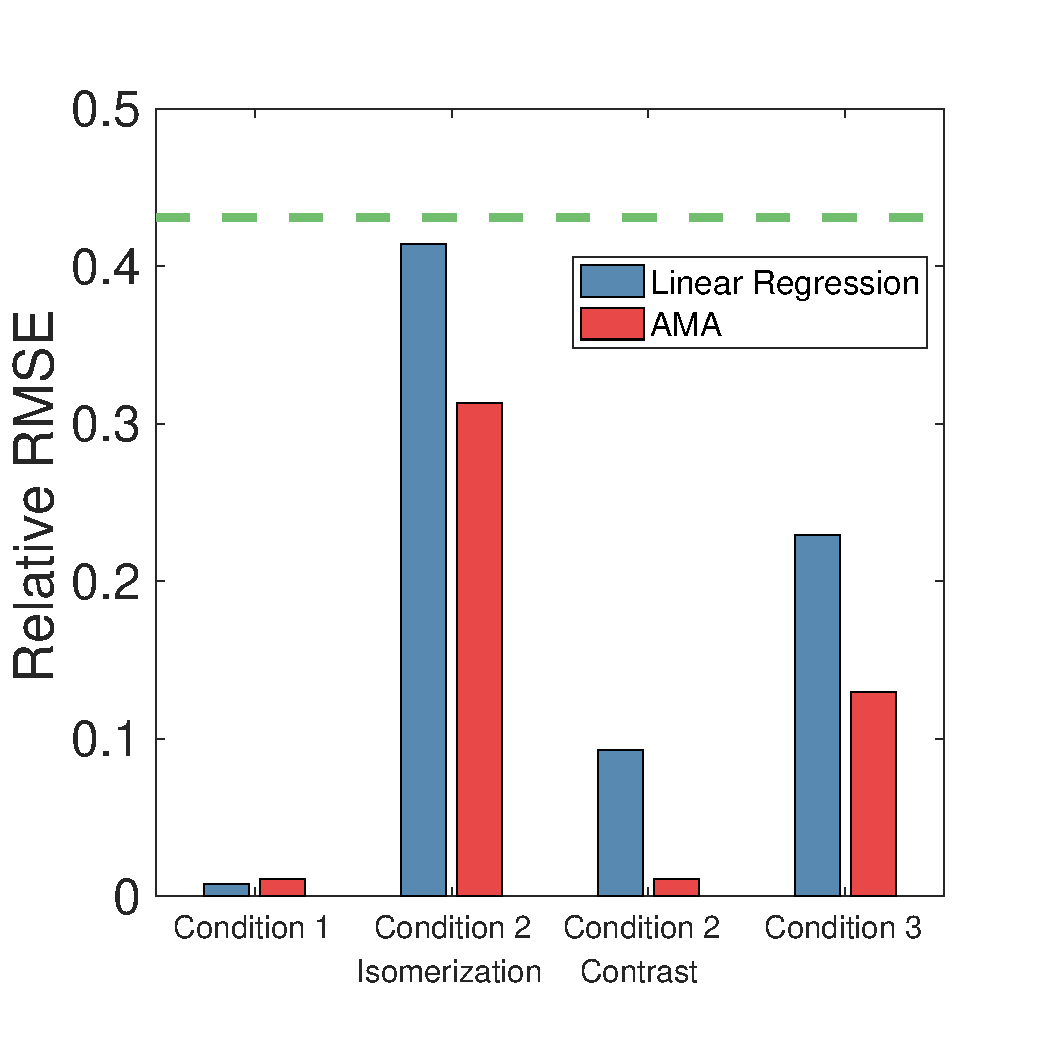
\includegraphics[width=0.3\textwidth]{../FiguresDraft4/Figure13/Figure13_a.pdf}
\caption{{\bf Comparison of LRV estimates:} Error estimates}
 \label{fig:barGraphs}
\end{figure}

\section{Discussion} \label{Discussion}
In this paper, we studied luminance constancy using naturalistic images.
We used a software pipeline, which was developed for this work, to render datasets of multispectral images from scene descriptions.
Because we rendered the images, we were able to label each image by the luminance reflectance value (LRV) of a target object.
Across images, we varied the LRV of the target object, its relative surface reflectance spectrum, 
the spectral power distributions of the light sources, and the reflectance spectra of the background objects in the scene.
These variations were based on statistical models of natural surface reflectance and illumination spectra.
We used the labeled datasets to learn estimators for target object LRV.
We studied the performance of these estimators as we systematically manipulated the 
spectral variations in the datasets.
We show that the target object LRV can be recovered almost perfectly if only the target 
object spectrum or the target object spectrum and the illuminant spectra varies.
In the first case, the LRV can be estimated from the cone isomerizations and in the second case 
from the cone isomerization contrast between the target and the background objects.
If, in addition, the background object spectra also vary, the cone contrast is no longer 
proportional to the target object LRV.
In this case, the AMA estimator we used in this work can predict the LRV to within ~13\% (relative RMSE).

The variability in the final condition results from changes in background object spectra, which affects the estimation in two ways.
First, it effects the estimation of cone contrast due to the variability in the background.
Second, it also effects the cone isomerizations corresponding to the target object through 
variability in secondary reflections from the background objects.
While the first effect can be minimized by a representative sampling of the background, 
the effect of secondary reflections can not be removed through simple manipulations.
This effect has largely been ignored in the field. 
We show that such effects are significant.

The reason such effects have been ignored is that we have lacked tools to quantify their effects.
In this regard, a major contribution of this work is the development of a computational package to
produce naturalistic images with precise control over factors defining the scene.
With this software we can systematically vary these factors and precisely quantify their effects on constancy.


% MOVE THIS TO DISCUSSION
%This general approach has been adopted by other labs for the study of computational estimation of optical flow (Baker et al., 2011) and is becoming increasingly popular (Kovacs, Bell, Snavely, & Bala, 2017), as well as for the generation of stimuli for the study of human perception (e.g., Boyaci, Maloney, & Hersh, 2003; Todd & Mingolla, 1983; Arend & Reeves, 1986; Johnston, Cumming, & Parker, 1993). Of course, success within the domain of graphics images does not guarantee smooth generalization to real natural images, a point we return to in the Discussion.
% \cite{baker2011database}  \cite{kovacs17shading} \citeNP{boyaci2003effect, todd1983perception, arend1986Simultaneous, johnston1993integration}
% Autonmous vehicle work - ask BAW 

\bibliography{references}
\bibliographystyle{jovcite}

\end{document}

